\documentclass[10pt,twocolumn,letterpaper]{article}


\usepackage{style/iccv}
\usepackage{adjustbox}
\usepackage{times}
\usepackage{epsfig}
\usepackage{graphicx}

%%%%%%%%%%%%%%%%%%%%%%%%%%%%%%%%
% GRAPHICS
%%%%%%%%%%%%%%%%%%%%%%%%%%%%%%%%
\usepackage{graphicx}
\usepackage{epsfig}
\usepackage{tikz}
\usetikzlibrary{positioning}
\usetikzlibrary{shapes}
\usetikzlibrary{fit}
\usetikzlibrary{calc}
\newcommand{\bb}[0]{
\vspace{-0.25cm}}
\newcommand{\volume}[4]{
\draw[step=1cm,black,very thin] (#1,#2) grid (#3,#4);
\draw[black,fill=gray,fill opacity=0.2] (#1,#2) -- (#1,#4) -- (#3,#4) -- (#3,#2) -- cycle;
}
\newcommand{\Cvolume}[5]{
\draw[step=1cm,gray,very thin] (#1,#2) grid (#3,#4);
\draw[draw=none,fill=#5,fill opacity=0.2] (#1,#2) -- (#1,#4) -- (#3,#4) -- (#3,#2) -- cycle;
}

%%%%%%%%%%%%%%%%%%%%%%%%%%%%%%%%
% MATH
%%%%%%%%%%%%%%%%%%%%%%%%%%%%%%%%
\usepackage{mathtools,amsfonts,amsmath,amssymb,amsthm}
\theoremstyle{plain}
\newtheorem{theorem}{Theorem}
\newtheorem{proposition}{Proposition}
\newtheorem{lemma}{Lemma}
\newtheorem{corollary}{Corollary}

%%%%%%%%%%%%%%%%%%%%%%%%%%%%%%%%
% OTHERS
%%%%%%%%%%%%%%%%%%%%%%%%%%%%%%%%
\usepackage{url}
% \usepackage{multirow}
% \usepackage{varwidth}
\usepackage{enumitem}
\usepackage{listings}
\usepackage[ruled,vlined]{algorithm2e}

%%%%%%%%%%%%%%%%%%%%%%%%%%%%%%%%
% COLORS
%%%%%%%%%%%%%%%%%%%%%%%%%%%%%%%%
\usepackage{xcolor}
\definecolor{codegreen}{rgb}{0,0.6,0}
\definecolor{codegray}{rgb}{0.5,0.5,0.5}
\definecolor{codeblack}{rgb}{0.,0.,0.}
\definecolor{codepurple}{rgb}{0.58,0,0.82}
\definecolor{backcolour}{rgb}{0.95,0.95,0.92}

\lstdefinestyle{mystyle}{
    backgroundcolor=\color{backcolour},   
    commentstyle=\color{codegreen},
    keywordstyle=\color{codeblack},
    numberstyle=\tiny\color{codegray},
    stringstyle=\color{codepurple},
    basicstyle=\ttfamily\footnotesize,
    breakatwhitespace=false,         
    breaklines=true,                 
    captionpos=b,                    
    keepspaces=true,                 
    numbers=left,                    
    numbersep=5pt,                  
    showspaces=false,                
    showstringspaces=false,
    showtabs=false,                  
    tabsize=2,
    aboveskip=0pt,
    belowskip=-3pt
}
\lstset{style=mystyle}


\usepackage[pagebackref=true,breaklinks=true,colorlinks,bookmarks=false]{hyperref}

\usepackage[capitalize]{cleveref}
\crefname{lemma}{lemma}{lemmas}
\Crefname{lemma}{Lemma}{Lemmas}
\crefname{thm}{theorem}{theorems}
\Crefname{corollary}{Corollary}{Corollaries}

\usepackage{style/math}

\usepackage[accsupp]{axessibility}

% \newcommand\note[1]{\textcolor{red}{#1}}

% \usepackage{xcolor}
\definecolor{coolblack}{RGB}{40, 40, 45}
\definecolor{coolwhite}{RGB}{160, 160, 160}
\definecolor{coolblue}{RGB}{65, 130, 205}
\pagecolor{coolblack}
\color{coolwhite}   
\PassOptionsToPackage{allbordercolors=coolblue,allcolors=coolblue,colorlinks=true}{hyperref}
\definecolor{coolred}{RGB}{200, 60, 100}
\renewcommand\note[1]{\textcolor{coolred}{#1}}

\iccvfinalcopy

\def\iccvPaperID{12534} % *** Enter the ICCV Paper ID here
\def\httilde{\mbox{\tt\raisebox{-.5ex}{\symbol{126}}}}

% Pages are numbered in submission mode, and unnumbered in camera-ready
\ificcvfinal\pagestyle{empty}\fi

\newcommand\blfootnote[1]{%
  \begingroup
  \renewcommand\thefootnote{}\footnote{#1}%
  \addtocounter{footnote}{-1}%
  \endgroup
}

\begin{document}

\title{Active Self-Supervised Learning:\\A Few Low-Cost Relationships Are All You Need}

\author{
Vivien Cabannes*\\
Meta AI
\and
Leon Bottou\\
Meta AI
\and
Yann Lecun\\
Meta AI
\and
Randall Balestriero*\\
Meta AI
}

\maketitle
\ificcvfinal\thispagestyle{empty}\fi

%%%%%%%%% ABSTRACT
\begin{abstract}


Over the past few years, there has been a significant amount of research focused on studying the ReLU activation function, with the aim of achieving neural network convergence through over-parametrization. However, recent developments in the field of Large Language Models (LLMs) have sparked interest in the use of exponential activation functions, specifically in the attention mechanism.

Mathematically, we define the neural function $F: \R^{d \times m} \times  \mathbb{R}^d \rightarrow \mathbb{R}$ using an exponential activation function. Given a set of data points with labels $\{(x_1, y_1), (x_2, y_2), \dots, (x_n, y_n)\} \subset \mathbb{R}^d \times \mathbb{R}$ where $n$ denotes the number of the data. Here $F(W(t),x)$ can be expressed as $F(W(t),x) := \sum_{r=1}^m a_r \exp(\langle w_r, x \rangle)$, where $m$ represents the number of neurons, and $w_r(t)$ are weights at time $t$. It's standard in literature that $a_r$ are the fixed weights and it's never changed during the training. We initialize the weights $W(0) \in \mathbb{R}^{d \times m}$ with random Gaussian distributions, such that $w_r(0) \sim \mathcal{N}(0, I_d)$ and initialize $a_r$ from random sign distribution for each $r \in [m]$.

Using the gradient descent algorithm, we can find a weight $W(T)$ such that $\| F(W(T), X) - y \|_2 \leq \epsilon$ holds with probability $1-\delta$, where $\epsilon \in (0,0.1)$ and $m = \Omega(n^{2+o(1)}\log(n/\delta))$. To optimize the over-parametrization bound $m$, we employ several tight analysis techniques from previous studies [Song and Yang arXiv 2019, Munteanu, Omlor, Song and Woodruff ICML 2022]. 

 

\end{abstract}

\blfootnote{*Equal contribution.}

%%%%%%%%% BODY TEXT
\section{Introduction}
%It has recently become apparent that the rapid delivery of a treatment could become a key element in some situations. This is the case for mobile tumors where the dose conformity may be impacted by interplay effects between the scanned beam and the movement of the tumor\cite{Lambert2005, Bert2008}. This is also the case for FLASH treatments.

Recent studies have shown that the use of very high dose rates would improve the protection of healthy tissues without compromising tumor control\cite{Favaudon2014, BUONANNO2019, MontayGruel2019}. However, the preclinical results are sometimes contradictory\cite{Venkatesulu2019, BEYREUTHER2019} and the underlying mechanism is not well understood yet\cite{Pratx2019, Spitz2019, LABARBE2020, JIN2020}. Preliminary findings suggest that a dose rate of at least 40 Gy/s is a critical prerequisite for the manifestation of the FLASH effect\cite{Favaudon2014}. Nevertheless, recent research indicates that this threshold may not be universal, and the degree of the effect may depend on the dose rate\cite{MONTAYGRUEL2017, Rothwell2022}. It also seems that there could be a minimum dose threshold\cite{Rothwell2022}.

State-of-the-art proton therapy relies on pencil beam scanning (PBS) to achieve excellent dose conformity. However, current PBS systems cannot deliver an intensity modulated proton therapy (IMPT) treatment with a FLASH dose rate. On the one hand, changing the beam energy from one layer to the other takes about 1 second. Consequently, the time to deliver a field can be around 20 seconds. On the other hand, several fields are generally required and the treatment can be fractionated over several days.

In the light of the above, current PBS systems must be adapted to enable FLASH treatments. The combined use of a single energy layer and a patient-specific range modulator would decrease the irradiation time and thus increase the dose rate while maintaining conformity, with minimal system modifications\cite{Rothwell2022}. The 3D range modulator typically consists of a collection of pyramids of different heights which transforms the pristine Bragg peaks into spread-out ones. The base of the range modulator is shaped to act as a range compensator to match the distal contour of the tumor. It has been shown that this set-up could easily achieve dose rate of at least 40 Gy/s\cite{Zhang2022, Liu2022}.

To plan a conformal PBS FLASH treatment it is therefore necessary to optimize a patient-specific range modulator and the weights of the PBS spots. Several methods have already been proposed\cite{Simeonov2022, Liu2022, Zhang2022}. Although different, they are based on two common principles:
\begin{enumerate}
    \item A Monte Carlo dose engine is used to create a dictionary of dose distributions from which the sizes of the slabs of the pyramids constituting the range modulator are computed. To this end, a reference IMPT plan is first optimized and the energy levels are converted into slabs of range shifter.
    \item The optimized range modulator is placed between the nozzle exit and the CT to calculate the dose influence matrix required for spot weight optimization.
\end{enumerate}

These studies have proved the feasability of using a single energy layer with a range modulator to deliver a dose to a complex target volume. However, one can regret that the optimization of the range modulators is akin to dose mimicking as it is not performed with respect to the constraints of the original IMPT plan. In addition, this optimizations require a complex simulation pipeline with an external dose engine.

We present a new approach which is different in two aspects.

First, the modulator geometry and spot weights are optimized directly with respect to dose constraints similar to state-of-the-art IMPT inverse planning. We assume that the geometry of the range modulator and the weights of the PBS spots are intrinsically linked and benefit from not being optimized separately. In a way, this is similar to IMPT optimization where it is not appropriate to select the final entries of the dose influence matrix before optimizing the spot weights. The best solution can only be obtained when considering all possible combinations of range modulators and spot weights.

Secondly, we do not use any priors on the geometry of the range modulator. In particular, we do not impose that it consists of pyramids. On the contrary, our range modulator has a pixelated geometry. It can be represented by an elevation map in raster form. Thus, the optimizer generates an optimal arbitrary geometry consisting eg. of truncated and non-symmetrical pyramids to better conform to the complex shape of the target volume. In addition, with such a voxelized geometry the range modulator can directly be added in the CT to perform dose calculations without having to resort to a tool supporting parameterized geometries.

The approache presented in this paper was applied to a head and neck case and compared to state-of-the-art IMPT.


\section{Methods}
\subsection{Overview of the treatment plan optimization process}
In classical inverse planning, the parameters subject to optimization are the spot weights $\bm{w}$. For conformal FLASH, we must also optimize the individual heights, named $\bm{h}$, of the range modulator which is coded as an elevation map as shown on Fig.~\ref{fig:schem_CEF}.

\begin{figure}[h]
    \centering
    \includegraphics[width=0.45\textwidth]{Schema_CEF.pdf}
    \caption{A 3D range modulator can be represented as a 2D elevation map. It is split into 'towers' and a range shifter. A minimum thickness of plain material is left attached to the 'towers' accordingly to 3D printing specification.}
    \label{fig:schem_CEF}
\end{figure}


Following a classical approach, the objectives penalize deviations of the dose from a reference value in a region of interest (ROI)\cite{Oelfke2001}. For example, to enforce a minimum dose named $D_{min}$, the following objective term may be minimized:
\begin{equation}
    f_{min}(\bm{w}, \bm{h}) = \frac{1}{N_r} \sum_{i=1}^{N_r} max_{\bm{w}, \bm{h}} \left( 0, D_{min} - D_i(\bm{w}, \bm{h}) \right)^2
    \label{eq:fmin}
\end{equation}
where $N_r = |ROI|$.

A similar objective may be used to enforce a maximum dose named $D_{max}$:
\begin{equation}
    f_{max}(\bm{w}, \bm{h}) = \frac{1}{N_r} \sum_{i=1}^{N_r} max_{\bm{w}, \bm{h}} \left( 0, D_i(\bm{w}, \bm{h}) - D_{max} \right)^2
    \label{eq:fmax}
\end{equation}
%
%Mean dose objectives can also be defined in a similar way but they are not developed in this paper for the sake of conciseness.

Several objectives may be defined. Hence, the general treatment plan optimization problem takes the following form:
\begin{eqnarray}
min && \sum_i f_i(\bm{w}, \bm{h})\label{eq:opti_problem}\\
 & s.t. & \bm{w} \geq 0 \nonumber\\
 & & \bm{h} \geq 0\nonumber
\end{eqnarray}
where $f_i(\bm{w}, \bm{h})$ are either of $f_{min}(\bm{w}, \bm{h})$ or $f_{max}(\bm{w}, \bm{h})$ -type.

A common approach for the minimization of Eq.~\ref{eq:opti_problem} with respect to $\bm{w}$ involves a dose influence matrix\cite{Oelfke2001}. Each column of this matrix is the dose contribution of one spot of the treatment plan. Hence, the total dose is computed as a weighted sum of the entries of the dose influence matrix. An analytical formulation of the derivative of the objective terms~\ref{eq:fmin} and~\ref{eq:fmax} can easily be calculated and fed to a first-order optimizer.

On the contrary, the minimization of Eq.~\ref{eq:opti_problem} with respect to $\bm{h}$ cannot be computed using a dose influence matrix. Instead, we propose to compute the derivative of the objetive terms by finite difference as described in details in section~\ref{sec:rm_opti}

The optimization over $\bm{w}$ and $\bm{h}$ is done iteratively as depicted on Fig.~\ref{fig:optimization_scheme}. Typical layouts are square or hexagonal grids. The optimization of $\bm{h}$ is nested in the optimization of $\bm{w}$. In other words, at each iteration of the optimization of $\bm{h}$, the spots weights $\bm{w}$ are fully re-optimized based on the current value of $\bm{h}$. This choice is a trade-off between the computation times of the two kinds of gradients. The evaluation of the gradient with respect to $\bm{h}$ requires a full computation by finite difference for each update of $\bm{h}$. Conversely, recomputing the gradient with respect to to $\bm{w}$ for new values of $\bm{w}$ is done based on the precalculated dose influence matrix which is must faster.

\begin{figure}
    \centering
    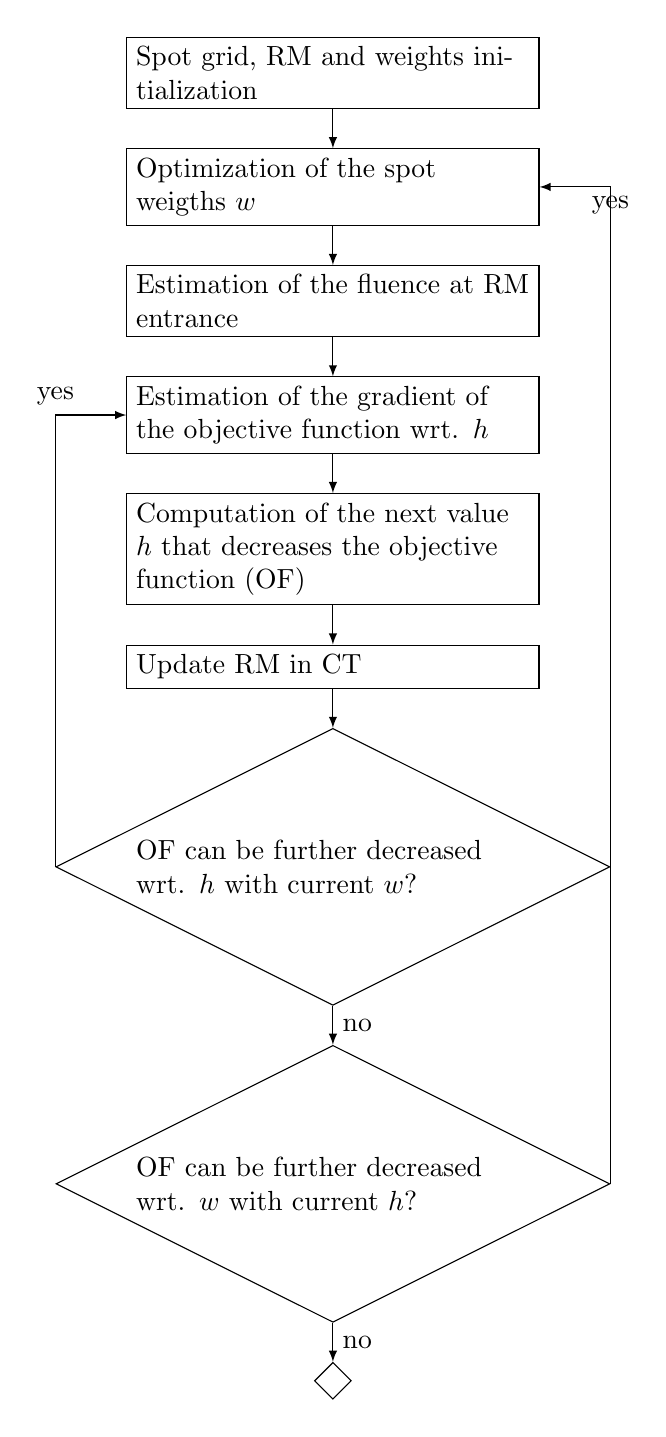
\begin{tikzpicture}
        \matrix [column sep=7mm, row sep=5mm] {
          \node (initialization) [draw, shape=rectangle, text width=5cm] {Spot grid, RM and weights initialization}; \\
          \node (weightOpti) [draw, shape=rectangle, text width=5cm] {Optimization of the spot weigths $\bm{w}$}; \\
          \node (fluence) [draw, shape=rectangle, text width=5cm] {Estimation of the fluence at RM entrance}; \\
          \node (gradient) [draw, shape=rectangle, text width=5cm] {Estimation of the gradient of the objective function wrt. $\bm{h}$}; \\
          \node (updateH) [draw, shape=rectangle, text width=5cm] {Computation of the next value $\bm{h}$ that decreases the objective function (OF)}; \\
          \node (updateCEM) [draw, shape=rectangle, text width=5cm] {Update RM in CT}; \\
          \node (coninueCEMOpti) [draw, diamond, aspect=2, text width=5cm] {OF can be further decreased wrt. $\bm{h}$ with current $\bm{w}$?};\\
          \node (coninueWOpti) [draw, diamond, aspect=2, text width=5cm] {OF can be further decreased wrt. $\bm{w}$ with current $\bm{h}$?};\\
          \node (done) [draw, diamond] {};\\
        };
        \draw[-latex] (initialization) edge (weightOpti);
        \draw[-latex] (weightOpti) edge (fluence);
        \draw[-latex] (fluence) edge (gradient);
        \draw[-latex] (gradient) edge (updateH);
        \draw[-latex] (updateH) edge (updateCEM);
        \draw[-latex] (updateCEM) edge (coninueCEMOpti);
        \draw[-latex, bend left] (coninueCEMOpti.west) |- node[auto] {yes} (gradient.west);
        \draw[-latex] (coninueCEMOpti) edge node[auto] {no}  (coninueWOpti);
        \draw[-latex, bend right] (coninueWOpti.east) |- node[auto] {yes} (weightOpti.east);
        \draw[-latex] (coninueWOpti) edge node[auto] {no}  (done);
        \end{tikzpicture}
    \caption{Schematics of the iterative optimization of the individual heights of the range modulator (RM) named $\bm{h}$ and the PBS spot weights named $\bm{w}$.}
    \label{fig:optimization_scheme}
\end{figure}

\subsection{Range modulator optimization\label{sec:rm_opti}}
For each iteration of the range modulator optimization, $\bm{w}$ is fixed and $\bm{h}$ remains the only variable to optimize on.

The gradient with respect to $\bm{h}$ of $f_{min}(\bm{w}, \bm{h})$ is:
\begin{equation}
    \nabla f_{min} = \frac{2}{N_r} \sum_{i=1}^{N_r} max_{\bm{h}} \left( 0, D_{min} - D_i(\bm{w}, \bm{h}) \right) \frac{\delta D_i(\bm{w}, \bm{h})}{\delta\bm{h}}
    \label{eq:grad_fmin}
\end{equation}
A similar gradient may be derived for $f_{max}$.

In Eq.~\ref{eq:grad_fmin}, the computation of $\frac{\delta D_i(\bm{w}, \bm{h})}{\delta\bm{h}}$ is a non trivial operation as the dose $D_i(\bm{w}, \bm{h})$ is usually computed with a Monte Carlo dose engine which does not provide any information of the variation of the particle range with respect to a small variation $\delta E$ of its initial energy. Computing the gradient by finite difference by running a simulation for every element of the vector $\delta \bm{h}$ may be intractable in terms of computation time but also in terms of memory because $|\bm{h}|$ simulations would have to be performed and stored. Therefore, we have adapted our Monte Carlo dose engine to perform and store computation not per beamlet but per pixel of an initial fluence map.

The derivative $\frac{\delta D_i(\bm{w}, \bm{h})}{\delta\bm{h}}$ is not directly estimated. Instead, we compute $\frac{\delta D_i(\bm{w}, \bm{h})}{\delta \bm{E}}$ where $\delta \bm{E}$ is the decrease in energy of the particles at the entrance of the range modulator caused by the increase in thickness $\delta\bm{h}$. It turns out in conformal FLASH that both derivatives are proportional since a single energy layer is used. Specifically, the relationship between the change in energy and in range is given by $\delta E = \delta h \times SP_{RM}(E)$, where $SP_{RM}(E)$ is the stopping power of the material used for the range modulator.

Our approach consists of providing a map of the fluence $\bm{F}$ at the entrance of the range modulator to a Monte Carlo dose engine which was modified to perform and store a simulation independently for each pixel of the fluence map. Those developments are detailed in section~\ref{sec:mcsquare}. For each pixel $h_j$ of the range modulator, we compute the dose $D(\bm{w}, \bm{h})$ for protons originating only at this location and with initial particles at nominal energy $E$. The number of protons is proportional to $F_j$. We then compute the dose $D(\bm{w}, \bm{h})$ in the exact same conditions but an initial energy of $E - \Delta E$. The derivative of $D_i(\bm{w}, \bm{h})$ may then be approximated as:
\begin{eqnarray}
    \frac{\delta D_{ij}(\bm{w}, h_j)}{\delta E} &=& \frac{\delta D_i(\bm{w}, E_j)}{\delta E_j} \\
    &\approx& \frac{D_i(\bm{w}, E_j) - D_i(\bm{w}, E_j - \Delta E_j)}{\Delta E_j}\label{eq:finite_diff}
\end{eqnarray}

Despite the modifications made in the dose calculator, the execution time may remain significant. To mitigate this, we propose a preliminary estimation of the objective function gradient using the continuous slowing down approximation (CSDA). Specifically, we estimate the dose in each voxel based on the energy loss calculated from a 3D map of relative proton stopping powers (RSPs) as follows:

\begin{eqnarray}
D_{x,y, z} &=& F_{x, y} SP_{w} \left( R(E_0) - \int RSP_{x, y, z} dz \right)
\end{eqnarray}

Here, $z$ is assumed to be along the beam direction, $SP_{w} (R(E))$ is the mass stopping power of water with respect to the range of protons having an energy equal to $E$, and $E_0$ is the nominal energy of the beam. While this approach neglects important phenomena like scattering and beam divergence, it can efficiently provide a rough estimate of $\mathbf{h}$. It is worth noting that this simple analytical approach often yields satisfactory results for the values of $\mathbf{h}$.

\subsection{Monte Carlo computations based on fluence map\label{sec:mcsquare}}
The Monte Carlo dose engine used in this study is MCsquare\cite{Souris2016} which takes advantage of mutli-core CPU architectures. MCsquare has the ability to compute the dose independently for each beamlet and store it in a sparse matrix without significant increase of the computation time. We hacked this feature to store the dose associated to each pixel of the range modulator.

MCsquare takes as input the location of the spot on the isocenter plane. To provide the fluence map to MCsquare, we first estimated the fluence at the entrance of the range modulator, given a model of the beam. Then, we projected the coordinates of the fluence values onto the isocenter plane given the distance between the steering magnets and the isocenter. Finally, the fluence map at isocenter was simply converted to the classical input taken by MCsquare.

Some modifications were made to the code of MCsquare to bypass its default sampling scheme. By default, MCsquare samples the initial particle locations according to a probability density function of which the parameters are defined in a beam model given as input. This default behavior was changed so that the initial location would be exactly the position of the pixels of the fluence map projected onto the plane of the nozzle exit.

In our modified MCsquare, the amount of particles to sample at each $(x, y)$ is now considered a deterministic variable corresponding to the pixels of the fluence map. The correlation between the particle direction and its location with respect to the center of the spot was also removed as such spots are not used anymore. Mathematically, MCsquare uses the following covariance matrix $\Sigma^2$ to sample the particles at the nozzle exit, for each beamlet:
\begin{equation}
\Sigma (z_{nozzle}) = 
  \begin{pmatrix}
    \sigma_x(z_{nozzle}) & \rho_{x \theta}(z_{nozzle})\\
    \rho_{x \theta}(z_{nozzle}) & \sigma_{\theta}(z_{nozzle})
  \end{pmatrix}  
\end{equation}
where $\sigma_x(z_{nozzle})$ is the standard deviation for the particle location, $\sigma_{\theta}(z_{nozzle})$ is the standard deviation for the particle direction and $\rho_{x \theta}$ is the correlation between particle position and direction. A similar covariance matrix is used for the y axis, de facto assuming no correlation between x and y.

However, when we provide the fluence at the nozzle exit, the initial location of the particle is now deterministic. It is constant for each pixel of the fluence map and therefore $\sigma_x(z_{nozzle})$ is zero. Consequently, it does not make sense anymore to consider any correlation between the particle direction and its constant initial location. The covariance matrix implemented in MCsquare was thus changed to:
\begin{equation}
\Sigma (z_{nozzle}) = 
  \begin{pmatrix}
    0 & 0\\
    0 & \sigma_{\theta}(z_{nozzle})
  \end{pmatrix}  
\end{equation}

\subsection{Optimization of the PBS spot weights}
The optimization of the spot weights is done classically as in Barragan~et~al.\cite{Barragan2018}. A dose influence matrix is first computed using MCsquare. The optimization problem~\ref{eq:opti_problem} is then solved by L-BFGS.

\subsection{Range modulator representation and insertion within the CT}
The range modulator is considered as a pixelated object which can be placed directly in the CT. The thickness in $(x, y)$ of the range modulator is encoded in a pixel value, as shown on Fig.~\ref{fig:schem_CEF}. In 3D, the range modulator can be seen as a collection of 'towers' attached to a plain area which can be considered as a range shifter. Those two kinds of components can be made in different materials. Although the use of plastic material for the range modulator fabrication would be convenient, a higher density material like aluminum could be chosen for the range shifter instead. This would serve to improve the lateral dose uniformity by increasing the amount of lateral scattering.

Splitting the range modulator into 'towers' and a range shifter is done dynamically at each iteration of the optimization. A minimum thickness of plain material is left attached to the 'towers' accordingly to 3D printing specifications which might be provided by the manufacturer. In this study this thickness was set to 5~mm.

To avoid resampling artefacts of the range modulators, all computations were done on CTs resampled on the beams-eye views. The CT resolution was $1\times1\times2~\mathrm{mm^3}$. Calculated dose maps were then resampled back on the original CT.

\subsection{Experimental validation}
To evaluate our optimization method, we used it to design conformal FLASH plans on an head and neck case. These plans were compared to conventional IMPT. Three PTVs were drawn as extentions of the CTVs: one on the left side and two on the right side of the patient. The prescriptions were 54.25~Gy for the left PTV and 54.25~Gy and 70~Gy for the two PTVs on the right side of the patient.

IMPT plans were optimized using RayStation~11b (RaySearch Laboratories, Stockholm, Sweden) considering four fields with gantry angles of around 60\degree, 120\degree, 240\degree, and 300\degree, and 10\degree couch rotation. A range shifter of 40 mm equivalent to water was used for all fields.

As FLASH treatments will most likely be hypofractionated\cite{Van_de_Water2019-pk} and a long delay might be required between the delivery of each field, setup errors might be critical. Designing the range modulator within a robust optimization framework would be highly desirable. However, this must be considered in a second instance after that the dose conformity which can be achieved with a range modulator is proved to be sufficient. Consequently, in the absence of a robust framework, the optimization of each field was done so as to have a uniform dose for that field. Given the shape of the target volume, it is clear that 120\degree and 240\degree are not appropriate to have a uniform dose. Therefore, those beam angles were not considered for FLASH treatment optimization which suggests that a different approach will have to be taken when planning FLASH treatments or to select patients eligible for a FLASH treatment.

A Python implementation of the aforementioned method was utilized to optimize FLASH plans. The maximum energy attainable from an IBA system, 226 MeV, was selected as the energy for the FLASH treatment. A spot size, characterized by a Gaussian distribution with standard deviations of $\sigma_x = 4.5$ mm and $\sigma_y = 5$ mm, was chosen. To account for the amplified scattering in the FLASH configuration, a spot spacing of 7~mm was employed in the present investigation.

The materials used for the range modulator, the range shifter and the collimator were respectively: PMMA (density: $1.2~\mathrm{g/cm^3}$), aluminum (density: $2.7~\mathrm{g/cm^3}$) and tungsten (density: $19.3~\mathrm{g/cm^3}$).


\section{Results\label{sec:results}}
\subsection{Dose conformity}
To evaluate our optimization method, we designed a conformal FLASH plan on an head and neck case. The target was composed of two rather large volumes, with irregular contours and variable depths. Fig.~\ref{fig:ptv7000_setup} shows the experimental setup and the dose distribution for the right part of the tumor.

\begin{figure}
    \centering
    \includegraphics[width=0.49\textwidth]{ptv7000_setup.png}
    \caption{Experimental setup for the right part of the tumor. From nozzle to patient: range modulator (PMMA), range shifter (aluminium), and aperture (tungsten).}
    \label{fig:ptv7000_setup}
\end{figure}

In this study, we mainly focused on the capabilities of the algorithm to give a uniform dose inside the target. We could not carry out an exhaustive dosimetric study as this head and neck case is not suitable for treatment with two opposite fields each giving a uniform dose. The combination of these fields would inevitably contribute to a superimposition of dose around the pharynx and therefore to a hot spot. In addition, a comprehensive dosimetric study should not only address differences in dose distributions but also take into account the benefits of using a high dose rate.

A Comparison with IMPT is shown on Fig.~\ref{fig:imptComparison5425} and~\ref{fig:imptComparison7000}. For the left PTV, the dose uniformity was close to IMPT. In the PTV we had $D95 = 52.5~\mathrm{Gy}$ and $D5 = 57.9~\mathrm{Gy}$ in FLASH, and $D95 = 51.8~\mathrm{Gy}$ and $D5 = 57.1~\mathrm{Gy}$ in IMPT. The dose was less uniform in the right PTV with $D95 = 65.2~\mathrm{Gy}$ and $D5 = 74.5~\mathrm{Gy}$ in FLASH, and $D95 = 67.3~\mathrm{Gy}$ and $D5 = 71.4~\mathrm{Gy}$ in IMPT. However, IMPT dose maps were obtained with two fields for each PTV whereas the FLASH treatment only had one field for each PTV.

To determine whether the degradation in dose uniformity was caused by the use of the range modulator or rather by the use of a single field and a large range shifter, we removed the range modulator from the CT and designed an IMPT plan with a single field. Fig.~\ref{fig:imptComparison7000}c shows the experimental setup: the range modulator was removed but the range shifter was left at the exact same place in the CT. The spot spacing used for that IMPT plan was the same as that used to design the FLASH plan. In Fig.~\ref{fig:imptComparison7000}d, the comparison of the dose profiles and the dose-volume histograms (DVHs) in the CTV shows that the design of the range modulator was actually very close to being optimal for these conditions, and that the dose degradation mainly came from the use of a single field and a large range modulator. D95s differ by $0.1~\mathrm{Gy}$ and D5s differ by $0.7~\mathrm{Gy}$.

\begin{figure*}
    \centering
    \includegraphics[width=\textwidth]{ptv5425_res_7mm.pdf}
    \caption{(a) Dose distribution obtained with the FLASH plan, (b) dose profile corresponding to a line passing through the center of the PTV, (c) IMPT dose distribution, and (d) DVH comparison for the left PTV and a prescription of 54.25~Gy.}
    \label{fig:imptComparison5425}
\end{figure*}

\begin{figure*}
    \centering
    \includegraphics[width=\textwidth]{ptv7000_res_impt_7mm.pdf}
    \caption{(a) Dose distribution obtained with the FLASH plan, (b) comparison of the corresponding DVH and that obtained in standard IMPT, (c) Dose distribution obtained with the single field IMPT plan and the same range shifter as for the FLASH plan, and (d) comparison of the corresponding DVH and that obtained in FLASH, in the CTV.}
    \label{fig:imptComparison7000}
\end{figure*}

\subsection{Dose rate}
In the current study, the PTVs considered had prescription doses of 54.5 Gy and 70 Gy. However, to accurately compute the dose rate, it is imperative to consider the dose per fraction, which is likely to be around 8~Gy for hypofractionated FLASH treatments. The spots were arranged in a conventional serpentine pattern, as depicted in Fig.~\ref{fig:drvh}c. The scanning speed was set at 8000 mm/s, and the current averaged on a pulse period was 500 nA at the nozzle output.

To assess the efficacy of a FLASH treatment, it is pertinent to evaluate the dose rate in the organs at risk (OARs) and the healthy tissues surrounding the target volume. However, to facilitate a direct comparison, a unique volume surrounding the PTV was defined instead of distinct volumes for each OAR. To delineate this volume, we first computed an extension of the PTV by 20 mm, named PTV-ext, which excluded areas where the dose was lower than 1 Gy.

The dose rate maps, along with the dose rate volume histograms (DRVHs), are presented in Fig.~\ref{fig:drvh}. It can be observed that the threshold of 40 Gy/s, commonly associated with the FLASH effect\cite{Favaudon2014}, is not achieved. Notably, the PBS dose rate is influenced by the length to be scanned in the primary scanning direction. Thus, the dose rate may potentially be enhanced through optimization of the scanning pattern.

\begin{figure*}
    \centering
    \includegraphics[width=\textwidth]{drvh_7mm.pdf}
    \caption{(a) and (b) Dose rate distribution computed for a current of 320 nA, (c) map of the intensity of the PBS spots, and (d) dose rate volume histogram.}
    \label{fig:drvh}
\end{figure*}

\section{Discussion}
The results presented in the previous section showed that the range modulators which were optimized for a complex head and neck case were optimal when considering dose uniformity and conformality.

One of the novel aspects in the proposed approach is that the range modulator is voxelized which has several advantages. First, it can be placed in the planning CT for dose computation. This greatly simplifies the simulation workflow as an external Monte Carlo dose engine supporting parameterized geometries like Geant4 do not need to be used. In addition, the geometry of the range modulator is arbitrarily set by the optimizer to optimally conform to the complex shape of the target volume. The algorithm is free to determine the height of each individual pixel of the elevation map and this typically results in asymmetrical pyramids as can be seen on the figures presented in Section~\ref{sec:results}.

Arbitrary geometry was not the sole improvement provided by the proposed method. Both the weights of the PBS spots and the individual heights of the range modulator were optimized directly under constraints. Thus, the range modulator was not optimized given spot weights but instead both spot weights and modulator elevations were updated at each iteration as dependent variables. This was possible thanks to the use of a fast Monte Carlo which could discriminate the contribution of each pixel of the range modulator.

In addition to the advantages just mentioned above, the proposed voxelized range modulator has a rather coarse resolution compared to other works in which it is similar to a conventional ridge filter with a high number of pyramidal peaks of variable prominence. The proposed range modulator typically has a resolution of around $1\times1\times1~\mathrm{mm^3}$. This is an asset for 3D printing. Even though current printing techniques have a precision of much less than one millimeter, this is not necessarily desirable from a mechanical point of view, in particular regarding the geometrical integrity in the presence of vibration or any externally applied force, including gravity.

In this first study, we compared a conformal FLASH plan to an IMPT plan optimized with a modern TPS considering robustness criteria. Conformal FLASH logically underperformed when compared to IMPT which comes from physical limitations, in particular the degradation of the distal fall off. However, we showed that the presented approach led to a dose distribution very close to that obtained with a single field IMPT and the same range shifter as that used for FLASH. The remaining slight difference could be explained by the fact that just as the range shifter degrades the sharpness of the Bragg peak, an additional degradation arises from the use of the range modulator. These observations makes it clear that the single field uniform dose approach considered in FLASH cannot compete with conventional IMPT in terms of dose conformity, and that should drive the selection of patient for FLASH treatments and the way that the plan would be designed. In addition, the optimization method could be integrated into a more complete approach, in particular with robustness criteria and a model of the FLASH effect on tumor control.

\section{Conclusions}
A joint range modulator and treatment plan optimization method was proposed and validated on an head an neck case. The optimization is done directly under constraints, similarly to IMPT inverse planning. The range modulator has a voxilized geometry which has many advantages: a simpler dose calculation pipeline, a geometry which can be arbitrarily determined by the optimizer and which is well suited for 3D printing.

\section{Acknowledgments}
This work was supported by the Walloon Region of Belgium through technology innovation partnership no. 8341 (EPT-1 – Emerging Proton Therapies Phase 1) co-led by MecaTech and BioWin clusters.

\section{Conflict of Interest Statement}
Dr. Kevin Souris was an employee of Ion Beam Applications during the writing of this paper.


{\small
\bibliographystyle{style/ieee_fullname}
\bibliography{references}
}

\onecolumn

\appendix
\input{appendix/active_learning}
\section{Proof of the main theorem}

Let $p$ be an odd prime and let $V$ be an $n$-dimensional vector space over $\mathbb{F}_p$ with basis $v_1,v_2,\dots,v_n$. The groups $G$ in (a),(b) are precisely those in (\ref{Gpi}), with $n=3$, associated to the linear maps
\begin{enumerate}[label = (\alph*)]
\item $\pi : V\rightarrow \Lambda^2V;\,$ $v_2^\pi = v_3^\pi  =1 $ and $v_1^\pi = (v_1\wedge v_2)$,
\item $\pi : V\rightarrow \Lambda^2V;\,$ $v_2^\pi = v_3^\pi =1 $ and $v_1^\pi = (v_2\wedge v_3)$.
\end{enumerate}
Similarly, the groups $G$ in (c),(d),(e) are precisely those in  (\ref{Gpi}), with $n=4$, associated to the linear maps
\begin{enumerate}[label = (\alph*)]\setcounter{enumi}{+2}
\item $\pi : V\rightarrow \Lambda^2V;\,$ $v_2^\pi = v_3^\pi = v_4^\pi =1 $ and $v_1^\pi = (v_1\wedge v_2)$,
\item $\pi : V\rightarrow \Lambda^2V;\,$ $v_2^\pi = v_3^\pi = v_4^\pi =1 $ and $v_1^\pi = (v_3\wedge v_4)$,
\item $\pi : V\rightarrow \Lambda^2V;\,$ $v_2^\pi = v_3^\pi = v_4^\pi =1 $ and $v_1^\pi = (v_1\wedge v_2)(v_3\wedge v_4)$.
\end{enumerate}
By Propositions \ref{rank one prop'} and \ref{rank one prop}, for $n=3,4$ and up to a change of basis, these are the only linear maps $\pi$ of rank one.

In this section, let us take $n=3,4$ and the symbol $\pi$ denotes one of the five linear maps above. As explained in Section \ref{group section}, we may identify
\[ G/G' = V\mbox{ and }G'=\Lambda^2V.\]
Moreover, we have a natural isomorphism
\[ \Aut^c(G) \simeq \Aut^c(\pi).\]
With these identifications, we may rephrase (\ref{Delta2}) as
\begin{equation}\label{Delta3}
\Delta(u^\alpha,v^\alpha) = \Delta(u,v)^{\hat{\alpha}}
\end{equation}
for all $u,v\in V$ and $\alpha\in\Aut^c(\pi)$. The $S$ and $S'$ in Section \ref{bilinear form sec} become
\begin{align*}
S &=  \{\mbox{symmetric bilinear $\Delta :V\times V\rightarrow \Lambda^2V$ satisfying (\ref{Delta3})}\}\\
S' &= \{\mbox{anti-symmetric bilinear  $\Delta :V\times V\rightarrow \Lambda^2V$ satisfying (\ref{Delta3})}\}
\end{align*}
in the current setting. The group $\Aut^c(\pi)$ was computed in Section \ref{group section}. Let $P$ and $Q$ denote the subgroups defined there. Then, we have
\[\Aut^c(\pi) = P\rtimes Q.\]
We shall also make the following assumption.

\begin{assume}Assume that $p\geq 5$ in the cases (a),(c),(e).
\end{assume}

We first show that the groups $G$ in question satisfy Assumption \ref{assumption} so that the discussion thereafter applies.  
\begin{lemma}\label{gamma lemma}
Let $\gamma : V\rightarrow\Aut^c(\pi)$ be an $\Aut^c(\pi)$-equivariant homomorphism and let $1\leq i,j\leq n$. Suppose that
\begin{enumerate}[label = $(\arabic*)$]
\item $\gamma(v_i)=1$,
\item $v_i^\alpha = v_iv_j$ for some $\alpha\in \Aut^c(\pi)$.
\end{enumerate}
Then $\gamma(v_j)=1$ also holds.
\end{lemma}

\begin{proof}Indeed, we have
\[ 1 = \gamma(v_i)^\alpha = \gamma(v_i^\alpha) = \gamma(v_i)\gamma(v_j) = \gamma(v_j)\]
by the hypotheses.
\end{proof}

\begin{prop}\label{gamma prop}There is no non-trivial $\Aut^c(\pi)$-equivariant homomorphism from $V$ to $\Aut^c(\pi)$.
\end{prop}

\begin{proof}Let $\gamma : V\rightarrow\Aut^c(\pi)$ be an $\Aut^c(\pi)$-equivariant homomorphism and observe that $\gamma(V)$ must be a normal $p$-subgroup of $\Aut^c(\pi)$. But
 \[ Q \simeq \begin{cases}
\mathbb{F}_p^\times\times \mathbb{F}_p^\times &\mbox{in case (a)}\\
\GL_2(\mathbb{F}_p)&\mbox{in cases (b) and (e)}\\
\mathbb{F}_p^\times \times \GL_2(\mathbb{F}_p)&\mbox{in cases (c) and (d)}
\end{cases}\]
has no non-trivial normal $p$-subgroup. Since $\Aut^c(\pi) = P\rtimes Q$, we see that $\gamma(V)$ must lie inside $P$. We now deal with each case separately.
\begin{enumerate}[label=(\alph*), wide=0pt]
\item It is clear from Proposition \ref{auto1'} that
\[ v_1^{\alpha_{12}} = v_1v_2\]
for some $\alpha_{12} \in P$, and so it is enough to show that $\gamma(v_1)=\gamma(v_3)=1$ by Lemma \ref{gamma lemma}, it. Let us put
\[ \gamma(v_1) = \begin{bmatrix}
1 & b_1 & 0 \\
0 & 1 & 0 \\
0 & c_1 & 1
\end{bmatrix}\mbox{ and }\gamma(v_3)= \begin{bmatrix}
1 & b_3 & 0 \\
0 & 1 & 0 \\
0 & c_3 & 1
\end{bmatrix} \]
From $\gamma(v_1^\alpha) = \gamma(v_1)^\alpha$ for $\alpha\in Q$ of the shape
\[ \alpha = \begin{bmatrix}s & 0 & 0 \\
0 & 1 & 0\\
0 & 0 & s\end{bmatrix} \mbox{ with } s\in \mathbb{F}_p^\times,\]
we get that $\gamma(v_1^\alpha) = \gamma(v_1)^s$ and
\[  \begin{bmatrix}
1 & sb_1 & 0 \\
0 & 1 & 0 \\
0 & sc_1 & 1
\end{bmatrix}= \begin{bmatrix}
1 & s^{-1}b_1 & 0 \\
0 & 1 & 0 \\
0 & s^{-1}c_1 & 1
\end{bmatrix}.\]
Since $p\geq 5$, there exists $s\in \mathbb{F}_p^\times$ with $s^2\neq 1$, and so $b_1=c_1=0$. We may obtain $b_3 = c_3 =0$ by the exact same calculation.
\item It is clear from Proposition \ref{auto2'} that
\[ v_1^{\alpha_{12}} = v_1v_2\mbox{ and } v_1^{\alpha_{13}} = v_1v_3\]
for some $\alpha_{12},\alpha_{13} \in P$, so it suffices to show that $\gamma(v_1)=1$ by Lemma \ref{gamma lemma}. Let us put
\[ \gamma(v_1) = \begin{bmatrix}1 & b_1 & c_1\\0& 1 & 0 \\ 0 & 0 & 1\end{bmatrix}.\]
From $\gamma(v_1^\alpha) = \gamma(v_1)^\alpha$ for $\alpha\in Q$ of the shape
\[\begin{bmatrix}
1 & 0 & 0\\
0 & s & 0\\
0 & 0 &s^{-1}
\end{bmatrix}\mbox{ with }s\in\mathbb{F}_p^\times,\]
we get that $\gamma(v_1^\alpha) = \gamma(v_1)$ and
\[  \begin{bmatrix}1 & b_1 & c_1\\0& 1 & 0 \\ 0 & 0 & 1\end{bmatrix}
=  \begin{bmatrix}1 & sb_1 & s^{-1}c_1\\0& 1 & 0 \\ 0 & 0 & 1\end{bmatrix}.\]
This yields $b_1=c_1=0$.
\item It is clear from Proposition \ref{auto1} that
\[ v_1^{\alpha_{12}} = v_1v_2\mbox{ and }v_3^{\alpha_{34}} = v_3v_4\]
for some $\alpha_{12}\in P, \alpha_{34}\in Q$, so it suffices to show that $\gamma(v_1)=\gamma(v_3)=1$ by Lemma \ref{gamma lemma}. Let us put
\[ \gamma(v_1) = \begin{bmatrix}
1 & b_1 & 0 & 0\\
0 & 1 & 0 & 0\\
0 & c_1 & 1 & 0\\
0 & d_1 & 0 & 1
\end{bmatrix}\mbox{ and }
 \gamma(v_3) = \begin{bmatrix}
1 & b_3 & 0 & 0\\
0 & 1 & 0 & 0\\
0 & c_3 & 1 & 0\\
0 & d_3 & 0 & 1
\end{bmatrix}.\]
From $\gamma(v_1^\alpha) = \gamma(v_1)^\alpha$ for $\alpha\in  Q$ of the shape
\[ \alpha =\begin{bmatrix}
s & 0 & 0 &0\\
0 & 1 & 0 & 0\\
0 & 0 & s & 0\\
0 & 0 & 0 & s
\end{bmatrix} \mbox{ with } s\in \mathbb{F}_p^\times,\]
we get that $\gamma(v_1^\alpha) = \gamma(v_1)^s$ and
\[ \begin{bmatrix}
1 & sb_1 & 0 & 0\\
0 & 1 & 0 & 0\\
0 & sc_1 &1 & 0\\
0 & sd_1 & 0 & 1
\end{bmatrix} = \begin{bmatrix}
1 & s^{-1}b_1 & 0 & 0\\
0 & 1 & 0 & 0\\
0 & s^{-1}c_1 &1 & 0\\
0 & s^{-1}d_1 & 0 & 1
\end{bmatrix} .\]
Since $p\geq 5$, there exists $s\in \mathbb{F}_p^\times$ with $s^2\neq 1$, and so $b_1=c_1=d_1=0$. We may obtain $b_3=c_3=d_3=0$ by the exact same calculation.
\item It is clear from Proposition \ref{auto2} that
\[ v_1^{\alpha_{12}} = v_1v_2,\,\ v_1^{\alpha_{13}} = v_1v_3,\,\ v_1^{\alpha_{14}} = v_1v_4.\]
for some $\alpha_{12},\alpha_{13},\alpha_{14}\in P$, and so it suffices to show that $\gamma(v_1)=1$ by Lemma \ref{gamma lemma}. Let us put
\[ \gamma(v_1) = \begin{bmatrix}
1 & b_1 & c_1 & e_1\\
0 & 1 & d_1 & f_1\\
0 & 0 & 1 & 0\\
0 & 0 & 0 & 1
\end{bmatrix}.\]
From $\gamma(v_1^\alpha) = \gamma(v_1)^\alpha$ for $\alpha\in \Aut^c(\pi)$ of the shape
\[ \alpha =\begin{bmatrix}
1 & 0 & 0 & 0\\
0 & 1 & g & 0\\
0 & 0 & s & 0\\
0 & 0 & 0 & s^{-1}
\end{bmatrix} \mbox{ with  } s\in \mathbb{F}_p^\times\mbox{ and }g\in \mathbb{F}_p,\]
we get that $\gamma(v_1^\alpha) = \gamma(v_1)$ and
\[ \begin{bmatrix}
1 & b_1 & c_1 & e_1\\
0 & 1 & d_1 & f_1\\
0 & 0 &1 & 0\\
0 & 0 & 0 & 1
\end{bmatrix} = \begin{bmatrix}
1 & b_1 & gb_1 + sc_1 & s^{-1}e_1\\
0 & 1 & sd_1 & s^{-1}f_1\\
0 & 0 & 1 & 0\\
0 & 0 & 0 &1 
\end{bmatrix}.\]
This yields $b_1 = c_1 = d_1=e_1=f_1=0$. 
\item It is clear from Proposition \ref{auto3} that
\[v_1^{\alpha_{12}} = v_1v_2,\,\ v_1^{\alpha_{13}} = v_1v_3,\,\ v_1^{\alpha_{14}} = v_1v_4\]
for some $\alpha_{12},\alpha_{13},\alpha_{14}\in P$, and so it suffices to show that $\gamma(v_1)=1$ by Lemma \ref{gamma lemma}. Let us put
\[ \gamma(v_1) = \begin{bmatrix}
1 & b_1 & -d_1 & c_1\\
0 & 1 & 0 & 0\\
0 & c_1 & 1 & 0\\
0 & d_1 & 0 & 1
\end{bmatrix}.\]
From $\gamma(v_1^\alpha) = \gamma(v_1)^\alpha$ for $\alpha\in Q$ of the shape
\[ \alpha =\begin{bmatrix}
s& 0 & 0 & 0\\
0 & 1 & 0 & 0\\
0 & 0 & s & 0\\
0 & 0 & 0 &1
\end{bmatrix} \mbox{ with } s\in \mathbb{F}_p^\times,\]
we get that $\gamma(v_1^\alpha) = \gamma(v_1)^{s}$ and
\[\begin{bmatrix}
1 & sb_1 & -sd_1 & sc_1\\
0 & 1 & 0 & 0\\
0 & sc_1 & 1 & 0\\
0 & sd_1 & 0 & 1
\end{bmatrix}= \begin{bmatrix}
1 & s^{-1}b_1 & -d_1 & s^{-1}c_1\\
0 & 1 & 0 & 0\\
0 & s^{-1}c_1 & 1 & 0\\
0 & d_1 & 0 & 1\end{bmatrix}.\]
This implies that $d_1=0$. Since $p\geq 5$, there exists $s\in \mathbb{F}_p^\times$ with $s^2\neq 1$, and we see that $b_1=c_1=0$ as well.
\end{enumerate}
In all cases, we have shown that $\gamma$ is trivial.
 \end{proof}
 
 Therefore, we may apply Theorem \ref{pre thm} to obtain
 \begin{equation}\label{T(G)} T(G) \simeq S \rtimes \res(\mathcal{S}').\end{equation}
It remains to determine the structure of $S$ and $\res(\mathcal{S}')$.

 \subsection{A module-theoretic approach} 
 
Observe that by the universal property of $S^2V$, the symmetric square of $V$, there is a natural correspondence between
\begin{itemize}
\item symmetric bilinear forms $V\times V\rightarrow\Lambda^2V$,
\item linear maps $S^2V\rightarrow \Lambda^2V$.
\end{itemize}
Similarly, there is a natural correspondence between
\begin{itemize}
\item anti-symmetric bilinear forms $V\times V\rightarrow\Lambda^2V$,
\item linear maps $\Lambda^2V\rightarrow \Lambda^2V$.
\end{itemize}
Since we are writing addition in $V$ multiplicatively, let us denote multiplication in $S^2V$ by $*$ to avoid confusion. Then, both $S^2V$ and $\Lambda^2V$ are naturally $\Aut^c(\pi)$-modules via the action
\[ (u* v)^{\alpha} = u^\alpha * v^\alpha\mbox{ and }(u\wedge v)^\alpha = u^\alpha \wedge v^\alpha\]
for all $u,v\in V$ and $\alpha\in \Aut^c(\pi)$. Taking (\ref{Delta3}) into account, it follows that elements of $S$ and $S'$, respectively, correspond to $\Aut^c(\pi)$-module homomorphisms $S^2V\rightarrow \Lambda^2V$ and $\Lambda^2V\rightarrow\Lambda^2V$.

Let us first restrict the action to $Q$. An $\Aut^c(\pi)$-module homomorphism is in particular a $Q$-module homomorphism. The latter is easier to understand because matrices in $Q$ are all block diagonal, and so we easily see that both $S^2V$ and $\Lambda^2V$, as $Q$-modules, are decomposable as a direct sum of irreducible submodules. In the tables below, we list a basis for each irreducible component, and we indicate the action of an arbitrary $\alpha\in Q$ in matrix form with respect to the given basis. Here
\[ \alpha = \begin{bmatrix} s & 0 & 0 \\ 0 & 1 & 0 \\ 0 & 0 &t\end{bmatrix},\begin{bmatrix}
|A| &  \begin{matrix} 0 & 0 \end{matrix}\\
 \begin{matrix} 0 \\ 0 \end{matrix} & A
\end{bmatrix}\]
in cases (a),(b), respectively, while 
\[ \alpha = \begin{bmatrix}
s & 0 & \begin{matrix} 0 & 0 \end{matrix}\\
0 & 1 & \begin{matrix} 0 & 0 \end{matrix}\\
\begin{matrix} 0 \\ 0 \end{matrix} & \begin{matrix} 0 \\ 0 \end{matrix} & A
\end{bmatrix},\begin{bmatrix}
|A| & 0 & \begin{matrix} 0 & 0 \end{matrix}\\
0 & s & \begin{matrix} 0 & 0 \end{matrix}\\
\begin{matrix} 0 \\ 0 \end{matrix} & \begin{matrix} 0 \\ 0 \end{matrix} & A
\end{bmatrix},\begin{bmatrix}
|A| & 0 & \begin{matrix} 0 & 0 \end{matrix}\\
0 & 1 & \begin{matrix} 0 & 0 \end{matrix}\\
\begin{matrix} 0 \\ 0 \end{matrix} & \begin{matrix} 0 \\ 0 \end{matrix} & A
\end{bmatrix}\]
in cases (c),(d),(e), respectively. The variables $s,t$ here range over $\mathbb{F}_p^\times$, and $A$ ranges over $\GL_2(\mathbb{F}_p)$.

 \begingroup
\setlength{\tabcolsep}{10pt} % Default value: 6pt
\renewcommand{\arraystretch}{1.15}
%\captionof{table}{}
 \begin{center}
  \begin{longtable}{ |c|c|}
  \multicolumn{2}{c}{Case (a)}\\
 \hline
 \hline
\multicolumn{2}{|c|}{Components of $S^2V$} \\
\hline
 Basis & Action of $\alpha\in Q$\\ \hline
 $v_1*v_1 $ & $s^2$ \\ 
 $v_1*v_2$ & $s$ \\ 
 $v_1*v_3$ & $st$ \\ 
 $v_2*v_2$ & $1$\\
 $v_2*v_3$ & $t$ \\
 $v_3*v_3$ & $t^2$\\
\hline\hline
\multicolumn{2}{|c|}{Components of $\Lambda^2V$}\\
\hline
 Basis & Action of $\alpha\in Q$ \\ \hline
 $v_1\wedge v_2 $ & $s$\\ 
 $v_1\wedge v_3$ & $st$  \\ 
 $v_2\wedge v_3$ & $t$\\ 
\hline
\end{longtable} 
 \begin{longtable}{ |c|c|}
  \multicolumn{2}{c}{Case (b)}\\
 \hline
 \hline
\multicolumn{2}{|c|}{Components of $S^2V$}\\
\hline
 Basis & Action of $\alpha\in Q$  \\ \hline
 $v_1*v_1 $ & $|A|^2$ \\ 
 $v_1*v_2,v_1*v_3$ & $|A|A$  \\ 
 $v_2*v_2, v_2*v_3,v_3*v_3$ & omitted  \\ 
\hline
\hline
\multicolumn{2}{|c|}{Components of $\Lambda^2V$}\\
\hline
 Basis & Action of $\alpha\in Q$ \\ \hline
 $v_1\wedge v_2 ,v_1\wedge v_3$ & $|A|A$  \\ 
 $v_2\wedge v_3$ & $|A|$  \\ 
\hline
\end{longtable}
 \begin{longtable}{ |c|c| }
  \multicolumn{2}{c}{Case (c)}\\
 \hline
 \hline
\multicolumn{2}{|c|}{Components of $S^2V$}\\
\hline
 Basis & Action of $\alpha\in Q$ \\ \hline
 $v_1*v_1 $ & $s^2$ \\ 
 $v_1*v_2$ & $s$ \\ 
 $v_1*v_3,v_1*v_4$ & $sA$  \\ 
 $v_2*v_2$ & $1$ \\
 $v_2*v_3,v_2*v_4$ & $A$ \\
 $v_3*v_3,v_3*v_4,v_4*v_4$ & omitted \\
\hline
\hline
\multicolumn{2}{|c|}{Components of $\Lambda^2V$} \\
\hline
 Basis & Action of $\alpha\in Q$  \\ \hline
 $v_1\wedge v_2 $ & $s$  \\ 
 $v_1\wedge v_3,v_1\wedge v_4$ & $sA$  \\ 
 $v_2\wedge v_3,v_2 \wedge v_4$ & $A$  \\ 
 $v_3\wedge v_4$ & $|A|$ \\
\hline
\end{longtable}
%\captionof{table}{The case when $v_1^\pi = v_1\wedge v_2$}\label{a sym}
 \begin{longtable}{ |c|c| }
 \multicolumn{2}{c}{Case (d)}\\
 \hline
 \hline
\multicolumn{2}{|c|}{Components of $S^2V$}\\
\hline 
Basis & Action of $\alpha\in Q$ \\ \hline
 $v_1*v_1 $ & $|A|^2$ \\ 
 $v_1*v_2$ & $s|A|$  \\ 
 $v_1*v_3,v_1*v_4$ & $|A|A$  \\ 
 $v_2*v_2$ & $s^2$\\
 $v_2*v_3,v_2*v_4$ & $sA$  \\
 $v_3*v_3,v_3*v_4,v_4*v_4$ & omitted \\
\hline
\hline
\multicolumn{2}{|c|}{Components of $\Lambda^2V$}\\
\hline 
Basis & Action of $\alpha\in Q$  \\ \hline
 $v_1\wedge v_2 $ & $s|A|$ \\ 
 $v_1\wedge v_3,v_1\wedge v_4$ & $|A|A$  \\ 
 $v_2\wedge v_3,v_2 \wedge v_4$ & $sA$  \\ 
 $v_3\wedge v_4$ & $|A|$ \\
\hline
\end{longtable}
%\captionof{table}{The case when $v_1^\pi = v_3\wedge v_4$}\label{a sym}
 \begin{longtable}{ |c|c| }
 \multicolumn{2}{c}{Case (e)}\\
 \hline
 \hline
\multicolumn{2}{|c|}{Components of $S^2V$}\\
\hline 
Basis & Action of $\alpha\in Q$ \\ \hline
 $v_1*v_1 $ & $|A|^2$ \\ 
 $v_1*v_2$ & $|A|$  \\ 
 $v_1*v_3,v_1*v_4$ & $|A|A$  \\ 
 $v_2*v_2$ & $1$ \\
 $v_2*v_3,v_2*v_4$ & $A$  \\
 $v_3*v_3,v_3*v_4,v_4*v_4$ & omitted \\
\hline
\hline
\multicolumn{2}{|c|}{Components of $\Lambda^2V$}\\
\hline 
Basis & Action of $\alpha\in Q$  \\ \hline
 $v_1\wedge v_2 $ & $|A|$ \\ 
 $v_1\wedge v_3,v_1\wedge v_4$ & $|A|A$  \\ 
 $v_2\wedge v_3,v_2 \wedge v_4$ & $A$  \\ 
 $v_3\wedge v_4$ & $|A|$  \\
\hline
\end{longtable}
%\captionof{table}{The case when $v_1^\pi = v_3\wedge v_4$}\label{a sym}
\end{center} 
\endgroup

\vspace{-0.55cm}
 
Under a $Q$-module homomorphism, an irreducible component of the domain either lies in the kernel or gets mapped to an isomorphic irreducible component of the codomain. From the stated action of $Q$, we can easily compare the isomorphism classes of the irreducible components of $S^2V$ and $\Lambda^2V$. Note that the omitted action does not matter because $\Lambda^2V$ does not have any $3$-dimensional irreducible component. The next two propositions are then immediate. 
 
 \begin{prop}\label{prelim prop sym}For any $\Delta\in S$, the following holds.
 \begin{enumerate}[label= $(\arabic*)$]
 \item In case (a), we have
\begin{align*}\Delta(v_1,v_1)&=1,\\
\Delta(v_2,v_2) &=1,\\
 \Delta(v_3,v_3)&=1.
\end{align*}
\item In case (b), we have
\begin{align*}
\Delta(v_1,v_1)& = 1,\\
\Delta(v_2,v_2) &= \Delta(v_2,v_3) =\Delta(v_3,v_3)=1.
\end{align*}
\item In cases (c),(d), and (e), we have
\begin{align*}
\Delta(v_1,v_1) &=1,\\
 \Delta(v_2,v_2) &=1,\\
 \Delta(v_3,v_3) &= \Delta(v_3,v_4)=\Delta(v_4,v_4) =1.
 \end{align*}
 \end{enumerate}
 \end{prop}
 
 \begin{prop}\label{prelim prop anti}
For any $\Delta\in S'$, the following holds.
 \begin{enumerate}[label= $(\arabic*)$]
\item In case (a), we have
\begin{align*}
\Delta(v_1,v_2) & \in \langle v_1\wedge v_2\rangle,\\
\Delta(v_1,v_3) & \in \langle v_1\wedge v_3\rangle,\\
\Delta(v_2,v_3) & \in \langle v_2\wedge v_3\rangle.
\end{align*}
\item In case (b), we have
\begin{align*}
\Delta(v_1,v_2),\Delta(v_1,v_3)& \in \langle v_1\wedge v_2,v_1\wedge v_3\rangle,\\
\Delta(v_2,v_3) & \in \langle v_2\wedge v_3\rangle.
\end{align*}
\item In cases (c) and (d), we have
\begin{align*}
 \Delta(v_1,v_2) & \in \langle v_1\wedge v_2\rangle,\\\
 \Delta(v_1,v_3),\Delta(v_1,v_4) & \in \langle v_1\wedge v_3, v_1\wedge v_4 \rangle,\\
 \Delta(v_2,v_3),\Delta(v_2,v_4) & \in \langle v_2\wedge v_3, v_2\wedge v_4 \rangle, \\
 \Delta(v_3,v_4) & \in \langle v_3\wedge v_4\rangle.
\end{align*}
\item In case (e), we have
\begin{align*}
 \Delta(v_1,v_2),\Delta(v_3,v_4) & \in \langle v_1\wedge v_2, v_3\wedge v_4\rangle,\\
 \Delta(v_1,v_3),\Delta(v_1,v_4) & \in \langle v_1\wedge v_3, v_1\wedge v_4 \rangle,\\
 \Delta(v_2,v_3),\Delta(v_2,v_4) & \in \langle v_2\wedge v_3, v_2\wedge v_4 \rangle
\end{align*}
\end{enumerate}  
 \end{prop}
  
We may refine parts of Proposition \ref{prelim prop anti} as follows.

 \begin{prop}\label{scalar prop} For any $\Delta\in S'$, the following holds.
 \begin{enumerate}[label= $(\arabic*)$]
 \item In case (b), there exists $\lambda\in\mathbb{F}_p$ such that
 \[ \begin{cases}
 \Delta(v_1,v_2) = (v_1\wedge v_2)^\lambda,\\
 \Delta(v_1,v_3) = (v_1\wedge v_3)^\lambda.
 \end{cases}\]
 \item In cases (c),(d), and (e), there exist $\lambda_1,\lambda_2\in \mathbb{F}_p$ such that
\[\begin{cases}
\Delta(v_1,v_3) = (v_1\wedge v_3)^{\lambda_1} \\
\Delta(v_1,v_4) = (v_1\wedge v_4)^{\lambda_1}
\end{cases}\,\
\begin{cases}
\Delta(v_2,v_3) = (v_2\wedge v_3)^{\lambda_2},\\
\Delta(v_2,v_4) = (v_2\wedge v_4)^{\lambda_2}.
\end{cases}\]
 \end{enumerate}
  \end{prop}
 
 \begin{proof} Consider case (b). We know from Proposition \ref{prelim prop anti} that $\Delta$ has to induce a $Q$-module endomorphism 
 \[ \delta : \langle v_1\wedge v_2,v_1\wedge v_3\rangle \rightarrow \langle v_1\wedge v_2,v_1\wedge v_3 \rangle.\]
If $\delta$ is trivial, then simply take $\lambda=0$. If $\delta$ is non-trivial, then it has to be invertible because $\langle v_1\wedge v_2,v_1\wedge v_3\rangle$ is irreducible. Say $\delta$ is given by the matrix $M\in \GL_2(\mathbb{F}_p)$. But $M$ must commute with the action of $Q$ and observe that $Q$ restricts to an $\SL_2(\mathbb{F}_p)$-action on $\langle v_1\wedge v_2,v_1\wedge v_3\rangle$.
Since the only matrices that centralize $\SL_2(\mathbb{F}_p)$ are the scalar multiples of the identity, it follows that $M = \left[\begin{smallmatrix} \lambda& 0\\ 0 & \lambda\end{smallmatrix}\right]$
for some $\lambda\in\mathbb{F}_p^\times$. The proves (1), and the same argument may be applied to prove (2).\end{proof}

\subsection{Computation of $S$ and $S'$} We shall now compute $S$ and $S'$ by taking the action of $P$ into account.

First, notice that a symmetric bilinear form $\Delta : V\times V\rightarrow \Lambda^2V$ is uniquely determined by
  \[ \Delta(v_i,v_j)\mbox{ for }1\leq i \leq j \leq n.\]
The next observation shall also be useful.

\begin{lemma}\label{sym lemma}Let $\Delta \in S$ and let $1\leq i, j \leq n$. If
\begin{enumerate}[label = $(\arabic*)$]
\item $\Delta(v_i,v_i) = \Delta(v_j,v_j)=1$,
\item  $v_i^{\alpha }= v_iv_j$ for some $\alpha\in \Aut^c(\pi)$,
\end{enumerate}
then $\Delta(v_i,v_j) =\Delta(v_j,v_i)= 1$ also holds.
\end{lemma}

\begin{proof}By the hypothesis and the condition (\ref{Delta3}), we have
\begin{align*}
1 & = \Delta(v_i,v_i)^{\hat{\alpha}}\\
& = \Delta(v_i^{\alpha} ,v_i^{\alpha})\\
& = \Delta(v_iv_j,v_iv_j)\\
& = \Delta(v_i,v_i)\Delta(v_i,v_j)\Delta(v_j,v_i)\Delta(v_j,v_j)\\
&=\Delta(v_i,v_j)\Delta(v_j,v_i)\\
& = \Delta(v_i,v_j)^2,
\end{align*}
where the last equality holds because $\Delta$ is symmetric. Since $p$ is odd, we may take the square root and so $\Delta(v_i,v_j)=\Delta(v_j,v_i)=1$.
\end{proof}

\begin{prop}\label{S=1} We have $S=1$ in all cases (a),(b),(c),(d), and (e).
\end{prop}

\begin{proof}Let $\Delta\in S$ be arbitrary. We consider each case separately.
\begin{enumerate}[label=(\alph*),wide=0pt]
\item It is clear from Proposition \ref{auto1'} that
\[ v_1^{\alpha_{12}} = v_1v_2\mbox{ and } v_3^{\alpha_{23}} = v_2v_3\]
for some $\alpha_{12},\alpha_{23}\in P$. We then have
\[ \Delta(v_i,v_j) = 1\mbox{ for all }1\leq i \leq j\leq 3\mbox{ with }(i,j)\neq (1,3) \]
by Proposition \ref{prelim prop sym} and Lemma \ref{sym lemma}. Comparing the irreducible components of $S^2V$ and $\Lambda^2V$ as $Q$-modules, we also see that
\[ \Delta(v_1,v_3) = (v_1\wedge v_3)^\lambda\]
for some $\lambda\in\mathbb{F}_p$. But consider the action of $\alpha\in P$ given by
\[ \alpha = \begin{bmatrix} 1 & 1 & 0 \\ 0 & 1 & 0 \\ 0 & 1 & 1\end{bmatrix}.\]
By the condition (\ref{Delta3}), we have
\begin{align*}
\Delta(v_1,v_3)^{\hat{\alpha}}  & = \Delta(v_1^\alpha,v_3^\alpha)\\
& = \Delta(v_1v_2,v_2v_3)\\
& = \Delta(v_1,v_2)\Delta(v_1,v_3)\Delta(v_2,v_2)\Delta(v_2,v_3)\\
& = \Delta(v_1,v_3).
\end{align*}
But the left hand side is equal to
\[(v_1v_2\wedge v_2v_3)^\lambda =  (v_1\wedge v_2)^\lambda  (v_2\wedge v_3)^\lambda\Delta(v_1,v_3).\]
It follows that $\lambda=0$ and so $\Delta(v_1,v_3)=1$ also holds.
\item It is clear from Proposition \ref{auto2'} that
\[ v_1^{\alpha_{12}} = v_1v_2\mbox{ and } v_1^{\alpha_{13}} = v_1v_3\]
for some $\alpha_{12},\alpha_{13}\in P$. We then have
\[ \Delta(v_i,v_j) = 1\mbox{ for all }1\leq i \leq j\leq 3 \]
by Proposition \ref{prelim prop sym} and Lemma \ref{sym lemma}. 
\item It is clear from Proposition \ref{auto1} that
\[ v_1^{\alpha_{12}} = v_1v_2,\, 
v_3^{\alpha_{23}} = v_2v_3,\, v_4^{\alpha_{24}} = v_2v_4\]
for some $\alpha_{12},\alpha_{23},\alpha_{24}\in P$. We then have
 \[ \Delta(v_i,v_j)=1\mbox{ for all }1\leq i \leq j \leq 4 \mbox{ with }(i,j)\not\in\{(1,3),(1,4)\}\]
by Proposition \ref{prelim prop sym} and Lemma \ref{sym lemma}. Comparing the irreducible components of $S^2V$ and $\Lambda^2V$ as $Q$-modules, we also see that
\[ \Delta(v_1,v_3),\Delta(v_1,v_4)\in \langle v_1\wedge v_3,v_1\wedge v_4\rangle\]
has to hold. Let us write
\[ \Delta(v_1, v_3) = (v_1\wedge v_3)^{\lambda}(v_1\wedge v_4)^{\kappa},\]
and consider the action of $\alpha_1\in P$ defined by
\[\alpha_1 =  \begin{bmatrix}1 & 1 & 0 & 0 \\
0 & 1 & 0 & 0\\
 0& 1 & 1 & 0\\
 0 & 0 & 0 & 1\end{bmatrix}.
 \]
Since $\Delta$ satisfies the condition (\ref{Delta3}), we get that
\begin{align*}
\Delta(v_1,v_3)^{\hat{\alpha}_1}
& = \Delta(v_1^{\alpha_1},v_3^{\alpha_1})\\
& = \Delta(v_1v_2,v_2v_3)\\
& =\Delta(v_1,v_2)\Delta(v_1,v_3)\Delta(v_2,v_2)\Delta(v_2,v_3)\\
& = \Delta(v_1,v_3).\end{align*}
But explicitly, the left hand side is given by
\[(v_1v_2\wedge v_2v_3)^\lambda (v_1v_2\wedge v_4)^{\kappa}  = (v_1\wedge v_2)^{\lambda} (v_2\wedge v_3)^\lambda(v_2\wedge v_4)^\kappa\Delta(v_1,v_3).\]
This shows that $\lambda = \kappa = 0$ and hence $\Delta(v_1,v_3) =1$. Since there exists $\alpha_2\in Q$ for which $v_1^{\alpha_2} = v_1$ and $v_3^{\alpha_2} = v_4$, we have
\[ 1 = \Delta(v_1,v_3)^{\hat{\alpha}_2} = \Delta(v_1^{\alpha_2},v_3^{\alpha_2} ) = \Delta(v_1,v_4).\]
We have thus shown that $\Delta(v_1,v_3) = \Delta(v_1,v_4)=1$ also holds.
\item It is clear from Proposition \ref{auto2} that 
\[ v_1^{\alpha_{12}} = v_1v_2,\,
v_1^{\alpha_{13}} = v_1v_3,\,
v_1^{\alpha_{14}} = v_1v_4,\,
v_2^{\alpha_{23}} = v_2v_3,\,
v_2^{\alpha_{24}} = v_2v_4\]
for some $\alpha_{12},\alpha_{13},\alpha_{14},\alpha_{23},\alpha_{24}\in P$. We then have
\[ \Delta(v_i,v_j) = 1\mbox{ for all }1\leq i \leq j\leq 4 \]
by Proposition \ref{prelim prop sym} and Lemma \ref{sym lemma}.  
\item It is clear from Proposition \ref{auto3} that
\[ v_1^{\alpha_{12}} = v_1v_2,\,
v_1^{\alpha_{13}} = v_1v_3,\,
v_1^{\alpha_{14}} = v_1v_4,\,
v_3^{\alpha_{23}} = v_2v_3,\,
v_4^{\alpha_{24}}= v_2v_4\]
for some $\alpha_{12},\alpha_{13},\alpha_{14},\alpha_{23},\alpha_{24}\in P$. We then have
\[ \Delta(v_i,v_j) = 1\mbox{ for all }1\leq i \leq j\leq 4 \]
by Proposition \ref{prelim prop sym} and Lemma \ref{sym lemma}.  
\end{enumerate}
In all cases, we have shown that $\Delta=1$, and so indeed $S=1$.
  \end{proof}
 
Next, note that an anti-symmetric bilinear form $\Delta :V \times V \rightarrow \Lambda^2V$ is uniquely determined by
\[ \Delta(v_i,v_j) \mbox{ for }1\leq i < j\leq n.\]
We also make the following observation.

\begin{lemma}\label{anti lemma}
Let $\Delta\in S'$ and let $1\leq i,j,k\leq n$ with $i\neq j,k$. If
\begin{enumerate}[label = $(\arabic*)$]
\item $\Delta(v_i,v_j) = (v_i\wedge v_j)^{\lambda_1}$ or equivalently $\Delta(v_j,v_i) = (v_j\wedge v_i)^{\lambda_1}$,
\item $\Delta(v_i,v_k) = (v_i\wedge v_k)^{\lambda_2}$ or equivalently $\Delta(v_k,v_i) = (v_k\wedge v_i)^{\lambda_2}$,
\item $v_i^\alpha = v_i,\, v_j^\alpha =v_jv_k$ for some $\alpha\in \Aut^c(\pi)$,\end{enumerate}
then $\lambda_1 = \lambda_2$ has to hold.
\end{lemma}

%Note that the equivalence holds because $\Delta$ is anti-symmetric.

\begin{proof}By the condition (\ref{Delta3}), we have
\[
\Delta(v_i,v_j)^{\hat{\alpha}} = \Delta(v_i^\alpha,v_j^\alpha)
= \Delta(v_i,v_jv_k)
=\Delta(v_i,v_j)\Delta(v_i,v_k). \]
Using the hypothesis, we rewrite this as
\[ (v_i\wedge v_j)^{\lambda_1}(v_i\wedge v_k)^{\lambda_1} = (v_i\wedge v_j)^{\lambda_1}( v_i\wedge v_k)^{\lambda_2},\] 
which implies that $\lambda_1 =\lambda_2$, as claimed.
\end{proof}

For each $\lambda\in\mathbb{F}_p$, as noted in Remark \ref{remark}, clearly
\[ \Delta_{[\lambda]} : V \times V\rightarrow \Lambda^2V;\,\ \Delta_{[\lambda]}(u,v) = (u\wedge v)^\lambda\]
is an anti-symmetric bilinear form satisfying (\ref{Delta3}), namely $\Delta_{[\lambda]}\in S'$.

\begin{prop}\label{S' prop}We have
\[ S' =\begin{cases}
  \{ \Delta_{[\lambda]} : \lambda\in \mathbb{F}_p\}&\mbox{in cases (a),(b),(c), and (d)},\\
  \{ \Delta_{[\lambda]}\Delta_{[\kappa]}^* : \lambda,\kappa\in \mathbb{F}_p\}&\mbox{in case (e)},
  \end{cases} \] 
where $\Delta_{[\kappa]}^* : V\times V\rightarrow \Lambda^2V$ denotes the anti-symmetric form defined by
\begin{align*}
\Delta_{[\kappa]}^*(v_1,v_2) & = (v_3\wedge v_4)^\kappa,&\Delta_{[\kappa]}^*(v_2,v_3) & = (v_2\wedge v_3)^{-\kappa},\\
\Delta_{[\kappa]}^*(v_1,v_3) & = (v_1\wedge v_3)^{-\kappa},&\Delta_{[\kappa]}^*(v_2,v_4)& = (v_2\wedge v_4)^{-\kappa},\\
\Delta_{[\kappa]}^*(v_1,v_4)& = (v_1\wedge v_4)^{-\kappa},&\Delta_{[\kappa]}^*(v_3,v_4) & = (v_1\wedge v_2)^{\kappa}.\end{align*}
\end{prop}

\begin{proof}Let $\Delta\in S'$ be arbitrary. We consider each case separately.
\begin{enumerate}[label=(\alph*),wide=0pt]
\item[(a),(b)] By Propositions \ref{prelim prop anti} and \ref{scalar prop}, we know that
\begin{align*} \Delta(v_1,v_2) &= (v_1\wedge v_2)^{\lambda_1}\\ 
\Delta(v_1,v_3) &= (v_1\wedge v_3)^{\lambda_2}\\
\Delta(v_2,v_3) &= (v_2\wedge v_3)^{\lambda_3}
\end{align*}
for some $\lambda_1,\lambda_2,\lambda_3 \in \mathbb{F}_p$. In case (a), by Proposition \ref{auto1'}, we have
\[ \begin{cases}
v_1^{\alpha_{12}} = v_1\\
v_3^{\alpha_{12}} = v_2v_3
\end{cases}\,\ \begin{cases}
v_3^{\alpha_{23}} = v_3\\
v_1^{\alpha_{23}} = v_1v_2
\end{cases}\]
for some $\alpha_{12},\alpha_{23}\in P$. In case (b), we already know from Proposition  \ref{scalar prop} that $\lambda_1=\lambda_2$, and by Proposition \ref{auto2'}, we have
\[ \begin{cases}
v_3^{\alpha_{23}} = v_3\\
v_1^{\alpha_{23}} = v_1v_2
\end{cases}\]
for some $\alpha_{23}\in P$. In both cases, we get that
\[\lambda :=\lambda_1 = \lambda_2 = \lambda_3\]
by Lemma \ref{anti lemma}. This shows that $\Delta = \Delta_{[\lambda]}$, as claimed.
\item[(c),(d)] By Propositions \ref{prelim prop anti} and \ref{scalar prop}, we know that
\begin{align*} \Delta(v_1,v_2) &= (v_1\wedge v_2)^{\lambda_1}&\Delta(v_2,v_3) & = (v_2\wedge v_3)^{\lambda_3}\\ 
\Delta(v_1,v_3) &= (v_1\wedge v_3)^{\lambda_2} & \Delta(v_2,v_4) &= (v_2\wedge v_4)^{\lambda_3}\\
\Delta(v_1,v_4) &= (v_1\wedge v_4)^{\lambda_2}&\Delta(v_3,v_4) &= (v_3\wedge v_4)^{\lambda_4}
\end{align*}
for some $\lambda_1,\lambda_2,\lambda_3,\lambda_4 \in \mathbb{F}_p$. In case (c), by Proposition \ref{auto1}, we have
\[ \begin{cases}
v_1^{\alpha_{12}} = v_1\\
v_3^{\alpha_{12}} = v_2v_3
\end{cases}\,\
\begin{cases}
v_3^{\alpha_{23}} = v_3\\
v_1^{\alpha_{23}} = v_1v_2
\end{cases}
\,\
\begin{cases}
v_4^{\alpha_{34}} = v_4\\
v_3^{\alpha_{34}} = v_2v_3
\end{cases}\]
for some $\alpha_{12},\alpha_{23},\alpha_{34}\in P$. In case (d), by Proposition \ref{auto2}, we have
\[ \begin{cases}
v_1^{\alpha_{12}} = v_1\\
v_2^{\alpha_{12}} = v_2v_3
\end{cases}\,\
\begin{cases}
v_3^{\alpha_{23}} = v_3\\
v_1^{\alpha_{23}} = v_1v_2
\end{cases}
\,\
\begin{cases}
v_4^{\alpha_{34}} = v_4\\
v_2^{\alpha_{34}} = v_2v_3
\end{cases}\]
for some $\alpha_{12},\alpha_{23},\alpha_{34}\in P$. In both cases, we get that 
\[\lambda :=\lambda_1 = \lambda_2 = \lambda_3= \lambda_4\]
by Lemma \ref{anti lemma}. This shows that $\Delta = \Delta_{[\lambda]}$, as claimed.
\item[(e)] By Propositions \ref{prelim prop anti} and \ref{scalar prop}, we know that 
\begin{align*} \Delta(v_1,v_2) &= (v_1\wedge v_2)^{\lambda_1}(v_3\wedge v_4)^{\kappa_1}&\Delta(v_2,v_3) & = (v_2\wedge v_3)^{\lambda_3}\\ 
\Delta(v_1,v_3) &= (v_1\wedge v_3)^{\lambda_2} & \Delta(v_2,v_4) &= (v_2\wedge v_4)^{\lambda_3}\\
\Delta(v_1,v_4) &= (v_1\wedge v_4)^{\lambda_2}&\Delta(v_3,v_4) &= (v_1\wedge v_2)^{\kappa_4}(v_3\wedge v_4)^{\lambda_4}
\end{align*}
 for some $\lambda_1,\lambda_2,\lambda_3,\lambda_4,\kappa_1,\kappa_4\in \mathbb{F}_p$. Consider $\alpha\in P$ given by
\[ \alpha = \begin{bmatrix} 1 & 0 & 0 & 1\\
0 & 1 & 0 & 0\\
 0 & 1 & 1 & 0 \\ 
 0 & 0 & 0 & 1\end{bmatrix},\]
and we compute that
 \begin{align*}
\Delta(v_1,v_2)^{\hat{\alpha}}& = (v_1v_4\wedge v_2)^{\lambda_1}(v_2v_3\wedge v_4)^{\kappa_1} \\
&= \Delta(v_1,v_2)(v_4\wedge v_2)^{\lambda_1-\kappa_1},\\
\Delta(v_1^\alpha,v_2^\alpha) & = \Delta(v_1v_4,v_2) \\
&=\Delta(v_1,v_2)(v_4\wedge v_2)^{\lambda_3},\\
\Delta(v_1,v_3)^{\hat{\alpha}} & = (v_1v_4\wedge v_2v_3)^{\lambda_2} \\
&= \Delta(v_1,v_3)(v_1\wedge v_2)^{\lambda_2}(v_4\wedge v_2)^{\lambda_2}(v_4\wedge v_3)^{\lambda_2},\\
\Delta(v_1^\alpha,v_3^\alpha) & = \Delta(v_1v_4,v_2v_3) \\
&= \Delta(v_1,v_3)(v_1\wedge v_2)^{\lambda_1-\kappa_4}(v_4\wedge v_2)^{\lambda_3}(v_4\wedge v_3)^{\lambda_4-\kappa_1},\\
\Delta(v_3,v_4)^{\hat{\alpha}} & = (v_1v_4\wedge v_2)^{\kappa_4}(v_2v_3\wedge v_4)^{\lambda_4}\\
& = \Delta(v_3,v_4)(v_2\wedge v_4)^{\lambda_4-\kappa_4},\\
\Delta(v_3^\alpha,v_4^\alpha) & = \Delta(v_2v_3,v_4)\\
&= \Delta(v_3,v_4)(v_2\wedge v_4)^{\lambda_3}.
\end{align*}
Since the condition (\ref{Delta3}) has to hold, we deduce that
\[ \lambda_3= \lambda_1 - \kappa_1,\,\
\lambda_2 = \lambda_1-\kappa_4 =\lambda_3=\lambda_4-\kappa_1,\,\ \lambda_3 = \lambda_4-\kappa_4.\]
Solving this system of equations, we get that
\[ \lambda := \lambda_1 = \lambda_4 ,\,\ \kappa:=\kappa_1=\kappa_4,\,\ \lambda_2 =\lambda_3 = \lambda -\kappa.\]
This shows that $\Delta = \Delta_{[\lambda]}\Delta_{[\kappa]}^*$. Conversely, for any $\lambda,\kappa\in\mathbb{F}_p$, we know that $ \Delta_{[\lambda]}\in S'$ already and it is straightforward to check that $\Delta_{[\kappa]}^*$ also satisfies (\ref{Delta3}), so then $\Delta_{[\lambda]}\Delta_{[\kappa]}^*\in S'$.
 \end{enumerate}
 This completes the proof.
\end{proof}
   
\subsection{The structure of $T(G)$} We shall now prove Theorem \ref{thm1}. We already know from (\ref{T(G)}) and Proposition \ref{S=1} that
\[ T(G) \simeq \res(\mathcal{S}').\]
In cases (a),(b),(c), and (d), the theorem follows because we have
\[ \res(\mathcal{S}') \simeq \mathbb{F}_p^\times\]
by Remark \ref{remark} and Proposition \ref{S' prop}. In case (e), by Proposition \ref{S' prop}, the elements of $S'$  are precisely the bilinear forms
\[ \Delta_{[\sigma]}: V\times V\rightarrow\Lambda^2V ;\,\  \Delta_{[\sigma]}(u,v) = (u\wedge v)^\sigma.\]
Here $\sigma$ is any endomorphism on $\Lambda^2V$ of the form
\begin{equation}\label{tau}
 \begin{bmatrix}
\lambda & &  & &&\kappa\\
 & \lambda-\kappa & & &&\\
 & & \lambda-\kappa & & &\\
 & & & \lambda-\kappa & &\\
 & & & &\lambda-\kappa &\\
\kappa & & & &&\lambda
\end{bmatrix} \mbox{ with }\lambda,\kappa\in \mathbb{F}_p,\end{equation}
written with respect to the basis
\[ v_1\wedge v_2, v_1\wedge v_3, v_1\wedge v_4,v_2\wedge v_3,v_2\wedge v_4,v_3\wedge v_4\]
of $\Lambda^2V$. By \cite[Example 3.4]{LMH}, we know that $N_{\Delta_{[\sigma]}}\simeq G$ occurs only for $1+2\sigma\in \GL(\Lambda^2V)$. Let us make a change of variables $\tau = 1+2\sigma$, and consider $\tau_{\lambda,\kappa}\in \GL(\Lambda^2V)$ of the form (\ref{tau}) but with the restriction $\kappa\neq\pm\lambda$. Observe that then
\[
\eta_{\lambda,\kappa}   = \begin{bmatrix}
\lambda+\kappa &&&\\
&(\lambda+\kappa)^{-1} &&\\
&&1&\\
&&&1
\end{bmatrix},\]
written with respect to the basis $v_1,v_2,v_3,v_4$ of $V$, in which case
\[\hat{\eta}_{\lambda,\kappa} = \begin{bmatrix}
1 &&&&&\\
 &\lambda+\kappa&&&&\\
 &&\lambda+\kappa&&&\\
 &&&(\lambda+\kappa)^{-1}&&\\
 &&&&(\lambda+\kappa)^{-1}&\\
 &&&&&1
\end{bmatrix},\]
yields a solution to $\pi\hat{\eta}_{\lambda,\kappa}\tau_{\lambda,\kappa} = \eta_{\lambda,\kappa}\pi$. From (\ref{S'}), we deduce that
\[ \res(\mathcal{S}') \simeq \{(\eta_{\lambda,\kappa},\hat{\eta}_{\lambda,\kappa}\tau_{\lambda,\kappa}) : \lambda,\kappa\in\mathbb{F}_p\mbox{ with }\kappa\neq\pm\lambda\}.  \]
It is straightforward to verify that
\[ \eta_{\lambda_{1},\kappa_1} \eta_{\lambda_{2},\kappa_{2}} = \eta_{\lambda,\kappa},\,\
 \hat{\eta}_{\lambda_1,\kappa_1}\tau_{\lambda_1,\kappa_1}\hat{\eta}_{\lambda_2,\kappa_2}\tau_{\lambda_2,\kappa_2} = \hat{\eta}_{\lambda,\kappa}\tau_{\lambda,\kappa}\]
 for any $\lambda_1,\lambda_2,\kappa_1,\kappa_2\in \mathbb{F}_p$ with $\kappa_1\neq\pm\lambda_1$ and $\kappa_2\neq\pm\lambda_2$, where
 \[\begin{bmatrix} \lambda & \kappa\\ \kappa &\lambda \end{bmatrix}= \begin{bmatrix} \lambda_1 &\kappa_1\\\kappa_1&\lambda_1\end{bmatrix}
 \begin{bmatrix}\lambda_2& \kappa_2\\ \kappa_2 & \lambda_2\end{bmatrix}
 =\begin{bmatrix} \lambda_1\lambda_2 + \kappa_1\kappa_2 & \lambda_1\kappa_2 +\lambda_2\kappa_1\\\lambda_1\kappa_2 +\lambda_2\kappa_1&\lambda_1\lambda_2 + \kappa_1\kappa_2 \end{bmatrix}.\]
It follows that $\res(\mathcal{S}')$ is isomorphic to the subgroup
\[ \left\{ \begin{bmatrix}\lambda & \kappa \\ \kappa & \lambda\end{bmatrix}  : \lambda,\kappa\in\mathbb{F}_p\mbox{ with }\kappa\neq\pm\lambda\right\}\]
of $\GL_2(\mathbb{F}_p)$, or conjugating by $\left[\begin{smallmatrix}1 & -1\\ 1 & 1 \end{smallmatrix}\right]$, the subgroup
\[ \left\{ \begin{bmatrix}\lambda + \kappa& 0 \\  0 & \lambda- \kappa\end{bmatrix}  : \lambda,\kappa\in\mathbb{F}_p\mbox{ with }\kappa\neq\pm\lambda\right\}\]
of $\GL_2(\mathbb{F}_p)$. This decomposes as
\[ \left\{ \begin{bmatrix} \lambda & 0 \\ 0 & 1 \end{bmatrix}: \lambda\in \mathbb{F}_p^\times \right\}\times  \left\{ \begin{bmatrix} 1 & 0 \\ 0 & \kappa \end{bmatrix}: \kappa\in \mathbb{F}_p^\times \right\}\]
and so is isomorphic to $\mathbb{F}_p^\times \times \mathbb{F}_p^\times$, as claimed in (e).
%We then have
%\begin{align*}
% \res(\mathcal{S'}) = & \{ (\eta,\hat{\eta}\tau)\Gamma(G) : \eta\in \GL(V),\, \tau\in \GL(\Lambda^2V)\\
% &\hspace{2.5cm}\mbox{of the shape (\ref{tau}) with $\kappa \neq \lambda,\pm2\lambda$,}\\
% &\hspace{2.5cm}\mbox{and the equation }\pi\hat{\eta}\tau = \eta\pi\mbox{ holds}\}
% \end{align*}
%by (\ref{res(S')}). Let us solve $\pi\hat{\eta}\tau = \eta\pi$ for such $\eta\in \GL(V)$ and $\tau\in \GL(\Lambda^2V)$ in a manner very similar to the proof of Proposition \ref{auto3}. Write 
%\begin{align*}
%v_1^\eta & = v_1^{n_{11}} v_2^{n_{12}} v_3^{n_{13}} v_4^{n_{14}}, \\
%v_2^\eta & = v_1^{n_{21}} v_2^{n_{22}} v_3^{n_{23}} v_4^{n_{24}},\\
%v_3^\eta & = v_1^{n_{31}} v_2^{n_{32}} v_3^{n_{33}} v_4^{n_{34}},\\
%v_4^\eta & = v_1^{n_{41}} v_2^{n_{42}} v_3^{n_{43}} v_4^{n_{44}}.
%\end{align*}
%Since $v_2^\pi =v_3^\pi = v_4^\pi = 1$, necessarily $n_{21} = n_{31} = n_{41} = 0$ and $n_{11}\neq0$. We may then simplify $v_1^{\pi\hat{\eta}\tau} = v_1^{\eta\pi}$ as
%\begin{align*}
%&((v_1^{n_{11}} v_2^{n_{12}} v_3^{n_{13}} v_4^{n_{14}} \wedge v_2^{n_{22}} v_3^{n_{23}} v_4^{n_{24}})( v_2^{n_{32}} v_3^{n_{33}} v_4^{n_{34}}\wedge v_2^{n_{42}} v_3^{n_{43}} v_4^{n_{44}}))^{\tau} \\
%&\hspace{7.25cm}= (v_1\wedge v_2)^{n_{11}} (v_3\wedge v_4)^{n_{11}}.\end{align*}
%Since $\langle v_1\wedge v_3\rangle$ and $\langle v_1\wedge v_4\rangle$
%are eigenspaces of $\tau$, which is taken to be invertible here, by comparing exponents, we see that $n_{23} = n_{24}=0$. and $n_{22}\neq0$. The above equation then becomes
%\begin{align*}
%&((v_1^{n_{11}} v_2^{n_{12}} v_3^{n_{13}} v_4^{n_{14}} \wedge v_2^{n_{22}})( v_2^{n_{32}} v_3^{n_{33}} v_4^{n_{34}}\wedge v_2^{n_{42}} v_3^{n_{43}} v_4^{n_{44}}))^{\tau} \\
%&\hspace{7.25cm}= (v_1\wedge v_2)^{n_{11}} (v_3\wedge v_4)^{n_{11}}.\end{align*}
%Since $\langle v_2\wedge v_3\rangle$ and $\langle v_2\wedge v_4\rangle$
%are eigenspaces of $\tau$, by comparing exponents, we similarly deduce that
%\[ -n_{13}n_{22} + \begin{vmatrix} n_{32} & n_{33} \\ n_{42} & n_{43} \end{vmatrix}
%= -n_{14}n_{22} + \begin{vmatrix} n_{32} & n_{34} \\ n_{42} & n_{44} \end{vmatrix} = 0.\]
%Finally, by comparing the $v_1\wedge v_2$ and $v_3\wedge v_4$ terms, we obtain
%\[ \begin{bmatrix}\lambda & \kappa \\ \kappa &\lambda\end{bmatrix}
%\begin{bmatrix}n_{11}n_{22} \\[4pt] \lvert\begin{smallmatrix} n_{33}&n_{34}\\n_{43}&n_{44}\end{smallmatrix}\rvert\end{bmatrix} 
%=\begin{bmatrix} n_{11}\\n_{11}\end{bmatrix}.\]
%The matrix on the left is taken to be invertible, so equivalently
%\[ \begin{bmatrix}n_{22}\\[4pt] n_{11}^{-1}\lvert\begin{smallmatrix} n_{33}&n_{34}\\n_{43}&n_{44}\end{smallmatrix}\rvert\end{bmatrix}=
%\begin{bmatrix} \lambda & \kappa \\ \kappa & \lambda\end{bmatrix}^{-1}\begin{bmatrix}1\\1\end{bmatrix} = \begin{bmatrix}(\lambda+\kappa)^{-1} 
%\\ (\lambda + \kappa)^{-1} 
%\end{bmatrix}.\]
%Put $s_{\lambda,\kappa} =\lambda +\kappa$. Then $\pi\hat{\eta}\tau = \eta\pi$ holds if and only if
%\begin{align*}
%\eta &= \begin{bmatrix}
%s_{\lambda,\kappa} \lvert\begin{smallmatrix}n_{33} & n_{34}\\n_{43} & n_{44}\end{smallmatrix}\rvert & n_{12} & s_{\lambda,\kappa} \lvert\begin{smallmatrix}n_{32} & n_{33} \\ n_{42} & n_{43}\end{smallmatrix}\rvert & s_{\lambda,\kappa} \lvert\begin{smallmatrix} n_{32} & n_{34} \\ n_{42} & n _{44}\end{smallmatrix}\rvert\\
%0 & s_{\lambda,\kappa}^{-1} & 0 & 0\\
%0 & n_{32} & n_{33} & n_{34}\\
%0 & n_{42} & n_{43} & n_{44}
%\end{bmatrix}\\
%& = \begin{bmatrix} s_{\lambda,\kappa} & 0 & 0& 0 \\
%0 & s_{\lambda,\kappa}^{-1}& 0 & 0 \\
% 0 & 0 & 1 & 0\\
% 0 & 0 & 0 & 1\end{bmatrix} \begin{bmatrix}
%\lvert\begin{smallmatrix}n_{33} & n_{34}\\n_{43} & n_{44}\end{smallmatrix}\rvert & s_{\lambda,\kappa}^{-1}n_{12} &\lvert\begin{smallmatrix}n_{32} & n_{33} \\ n_{42} & n_{43}\end{smallmatrix}\rvert & \lvert\begin{smallmatrix} n_{32} & n_{34} \\ n_{42} & n _{44}\end{smallmatrix}\rvert \\
%0 & 1 & 0 & 0\\
%0 & n_{32} & n_{33} & n_{34}\\
%0 & n_{42} & n_{43} & n_{44}
%\end{bmatrix},
%\end{align*}
%where this last matrix lies in $\Aut^c(\pi)$ by Proposition \ref{auto3}. The class of $(\eta,\hat{\eta}\tau)$ modulo $\Gamma(G)$ is not affected when $\eta$ is multiplied by an element of $\Aut^c(\pi)$. Thus, we may take
%\[ \eta = \begin{bmatrix} s_{\lambda,\kappa} &  & &  \\
% & s_{\lambda,\kappa}^{-1}&  &  \\
%  &  & 1 & \\
%  &  &  & 1\end{bmatrix},\,\ \hat{\eta} =
%\begin{bmatrix}
%  1 & & & & & \\
%  & s_{\lambda,\kappa}& &  &\\
%  &  & s_{\lambda,\kappa} & & &\\
%  & & & s_{\lambda,\kappa}^{-1} & &\\
%   &  & & &s_{\lambda,\kappa}^{-1} & \\
%  & &  & & & 1
%  \end{bmatrix}.\]
%% in which case we have
%% \begin{align*}
%%  \hat{\eta}\tau  =
%%\begin{bmatrix}
%%  \lambda & 0 & 0 & 0 & 0 &\kappa\\
%%  0 & (\lambda-\kappa)s_{\lambda,\kappa}& 0 & 0 &0 & 0\\
%%  0 & 0 & (\lambda-\kappa)s_{\lambda,\kappa} & 0 & 0 &0\\
%%  0 & 0 & 0 & (\lambda-\kappa)s_{\lambda,\kappa}^{-1}   & 0 & 0\\
%%   0 & 0 & 0 & 0 &(\lambda-\kappa)s_{\lambda,\kappa}^{-1} & 0 \\
%%\kappa & 0 & 0 & 0 & 0 & \lambda
%%\end{bmatrix}.
%%   \end{align*}
%To simplify notation, let us put
%\begin{align*}
%M_{\lambda,\kappa} & =  \left[ \begin{smallmatrix} \lambda + \kappa&&&\\ & (\lambda+\kappa)^{-1} &&\\ &&1&&\\&&&1\end{smallmatrix}\right],\\
% N_{\lambda,\kappa} & =  \left[\begin{smallmatrix}
% \lambda &&&&&\kappa\\
% & (\lambda-\kappa)(\lambda+\kappa) &&&&\\
% &&(\lambda-\kappa)(\lambda+\kappa) &&&\\\
% &&&(\lambda-\kappa)(\lambda+\kappa)^{-1}&&\\
% &&&&(\lambda-\kappa)(\lambda+\kappa)^{-1}&\\
%\kappa &&&&&\lambda
%\end{smallmatrix} \right].
%\end{align*}
%We then deduce that
%\[ \res(\mathcal{S}') \simeq \{ (M_{\lambda,\kappa} ,N_{\lambda,\kappa}) : \lambda,\kappa\in \mathbb{F}_p\mbox{ with }\kappa\neq \lambda,\pm2\lambda\},\]
%and it is not hard to show that this is isomorphic to 
\section{Implementation}
\label{sec:impl}

At \company, we have deployed \sysname in our internal clusters to serve daily DL workloads.
The internal clusters consist of heterogeneous GPUs, including NVIDIA T4 GPU and NVIDIA A10 GPU.
Integrated with Kubernetes~\cite{k8s}, \sysname manages thousands of GPUs in each cluster and more than 20,000 GPUs in all.

\parabf{Service manager.}
For online workloads, we use the existing service manager at \company which deploys containers, discovers service, and autoscales horizontal pods.

\parabf{Global manager.}
We modify the Kubernetes scheduler to schedule offline workloads.
The workload profiler takes several dedicated GPUs, whose number is negligible to the total number of GPUs.
When a new offline workload comes, the workload profiler performs a few dry runs of the workload and utilizes the NVIDIA Data Center GPU Manager (DCGM) tools~\cite{dcgm} and NVIDIA Management Library (NVML)~\cite{nvml} libraries to collect GPU metrics.
We collect about 2,000 data for each GPU type to train the speed predictor.
The MLPs of the speed predictor have four layers with hidden size $64\times 64$.
The MLPs are trained with momentum SGD optimizer~\cite{ruder2016overview} in PyTorch v1.8.0~\cite{paszke2019pytorch} until they converge.
\sysname invokes the scheduler periodically to schedule all offline workloads.
When moving workloads, we record checkpoints of offline workloads and restart the workloads after transmitting the models and checkpoints.
As the datasets are usually colossal, we store the datasets in a remote file system and fetch data during the execution.
We implement the scheduler as a third-party plugin to the Kubernetes scheduler.


\parabf{Local executor.}
Each local executor executes online workloads according to the service manager and offline workloads according to the global manager.
DL workloads are executed in Docker containers with our customized components.
We add Best-Effort GPU DevicePlugin in Kubernetes and relevant control paths with Kubelet and \sysprobe for offline workloads.
To control SM percentage, we leverage the environment variable $CUDA\_MPS\_ACTIVE\_THREAD\_PERCENTAGE$ provided by MPS.
The GPU monitor collects resource metrics through DCGM~\cite{dcgm} and NVML~\cite{nvml} for NVIDIA GPU.
The \sysprobe updates the state machine with the collected resource metrics and empirically-set thresholds.
When the state is unhealthy, the \sysprobe will ask the NodeManager in Kubernetes to evict offline workloads.
\bytecuda intercepts nearly 800 CUDA driver APIs for GPU memory allocation and kernel launch.
The GPU memory quota of offline workloads is fixed to $40\%$ as Figure~\ref{fig:motiv_gpu_resource} reports that most online workloads use less than $60\%$ GPU memory.
We adopt the cpuset of Cgroup for CPU isolation.
For memory, \sysname will evict offline workloads if memory usage is higher than a threshold or the kernel swap daemon is busy for a long time.
The parameters to calculate GPU load in Equation~\ref{equ:gpu_load}$\&$\ref{equ:clock_factor} are empirically selected through trial-and-error.


\end{document}